\documentclass[16pt]{report}

\usepackage[utf8]{inputenc}
\usepackage{graphicx}
\usepackage{graphics}
\usepackage{float}
\usepackage{verbatim}
\usepackage[boxed]{algorithm2e}
\usepackage[nottoc,numbib]{tocbibind}
\usepackage{amsmath}
\usepackage{setspace}
\setstretch{1.2}
\usepackage{hyperref}
\usepackage{listings}
\usepackage{amsmath}
\usepackage{amssymb}
\hypersetup{%
  colorlinks = true,
  linkcolor  = black
}
\hypersetup{
    colorlinks=false,
    pdfborder={0 0 0},
}
\setcounter{tocdepth}{4}
\setcounter{secnumdepth}{4}

\pagenumbering{Roman}
\begin{titlepage}
\begin{center}
    {\LARGE \textbf{Coordination of Synchronous Components with Time Triggered Programming
} }\\[2mm]
    \vspace{6.5mm}
    {\large \textbf{Seminar Report}}\\[5pt]
    {\large \textit{Submitted in partial fulfillment of requirements for the degree of}}\\[5pt]
    {\large \textbf{Master of Technology}}\\
    {\large \textbf{Computer Science and Engineering}}\\
    \vspace{6.5mm}
    {\large By}\\
    \vspace{3mm}
    {\large\textbf{Avais Ahmad}}\\
    {\large\textbf{173050043}}\\
    \vspace{6.5mm}
    {\large \textit{Guided By }}\\[5pt]
    {\large\textbf{Prof. Paritosh K. Pandya}}\\
    {\large\textbf{Prof. Kavi Arya}}\\
    \vspace{11mm}
    
\includegraphics[scale=0.4]{logo.png}\\
    \vspace{6mm}
    {\large Department of Computer Science and Engineering\\
    \textsc{Indian Institute of Technology, Bombay}}\\
    \vspace{11mm}
    \vspace{9mm}
    {\large\textsc{July, 2019}}
    \vspace{12mm}
\end{center}

\end{titlepage}

\begin{document}


\begin{figure}[H]
\centering
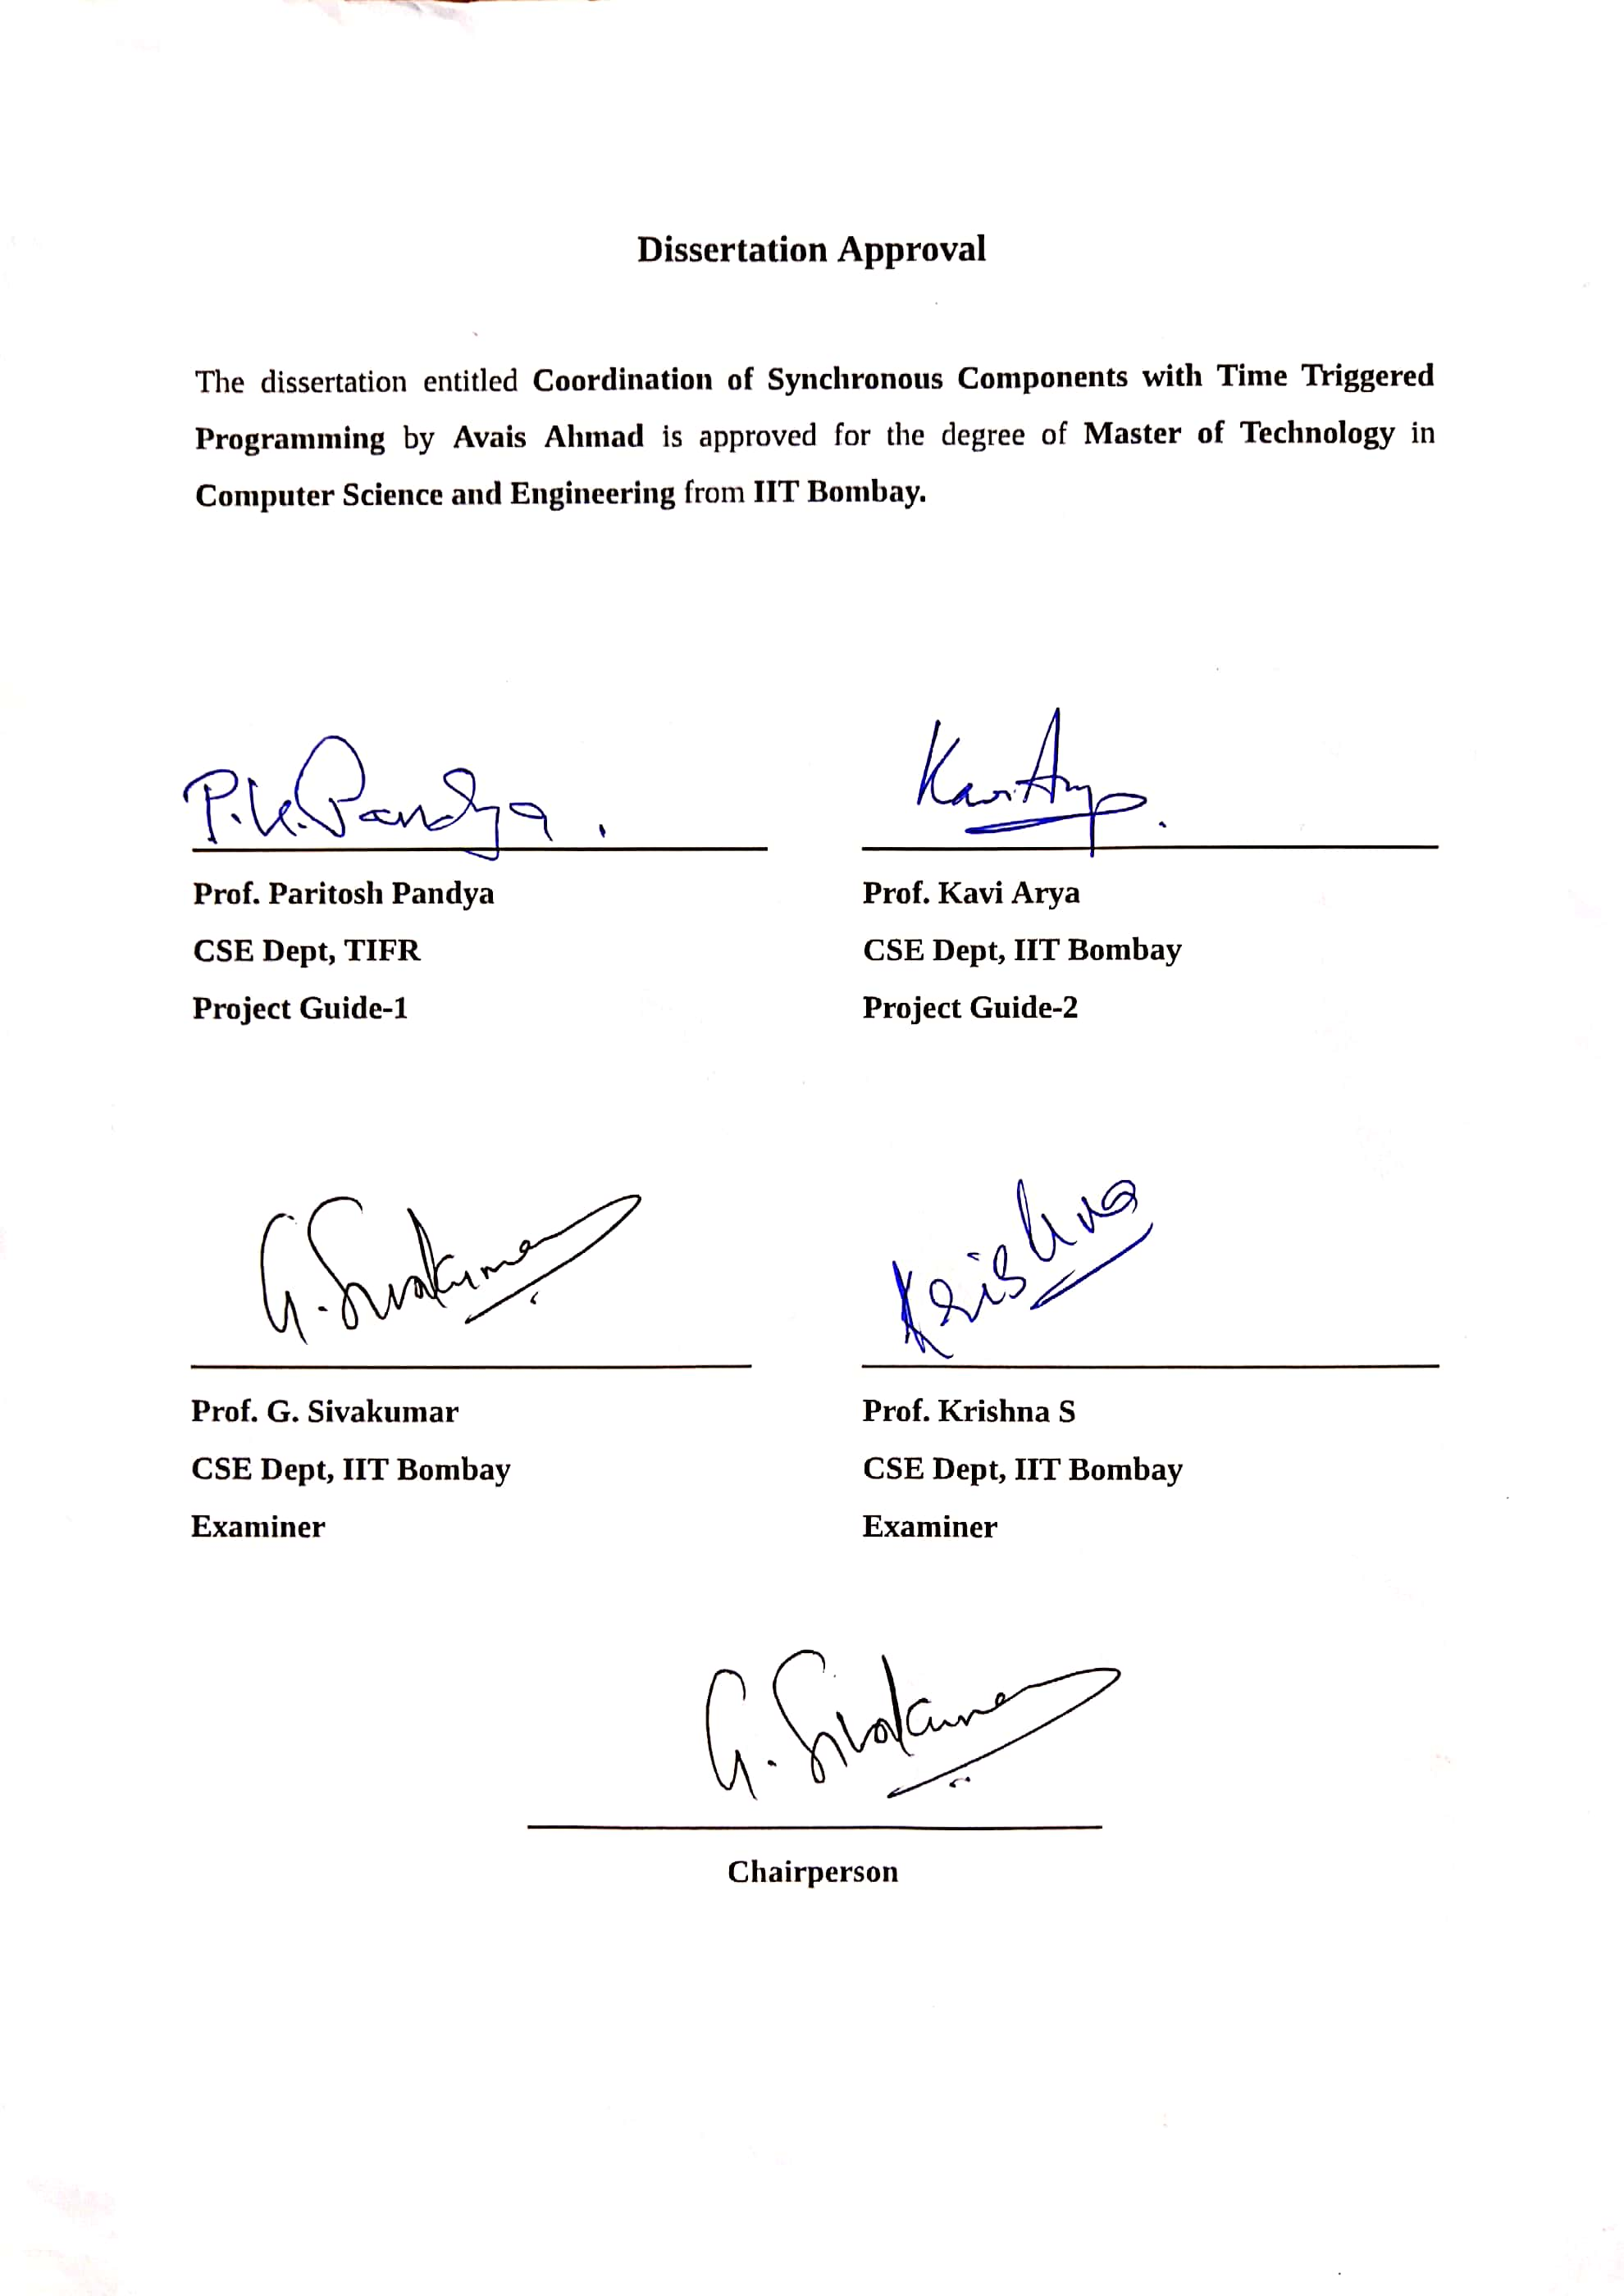
\includegraphics[width=\linewidth]{declaration.jpg}
\end{figure}

\begin{figure}[H]
\centering
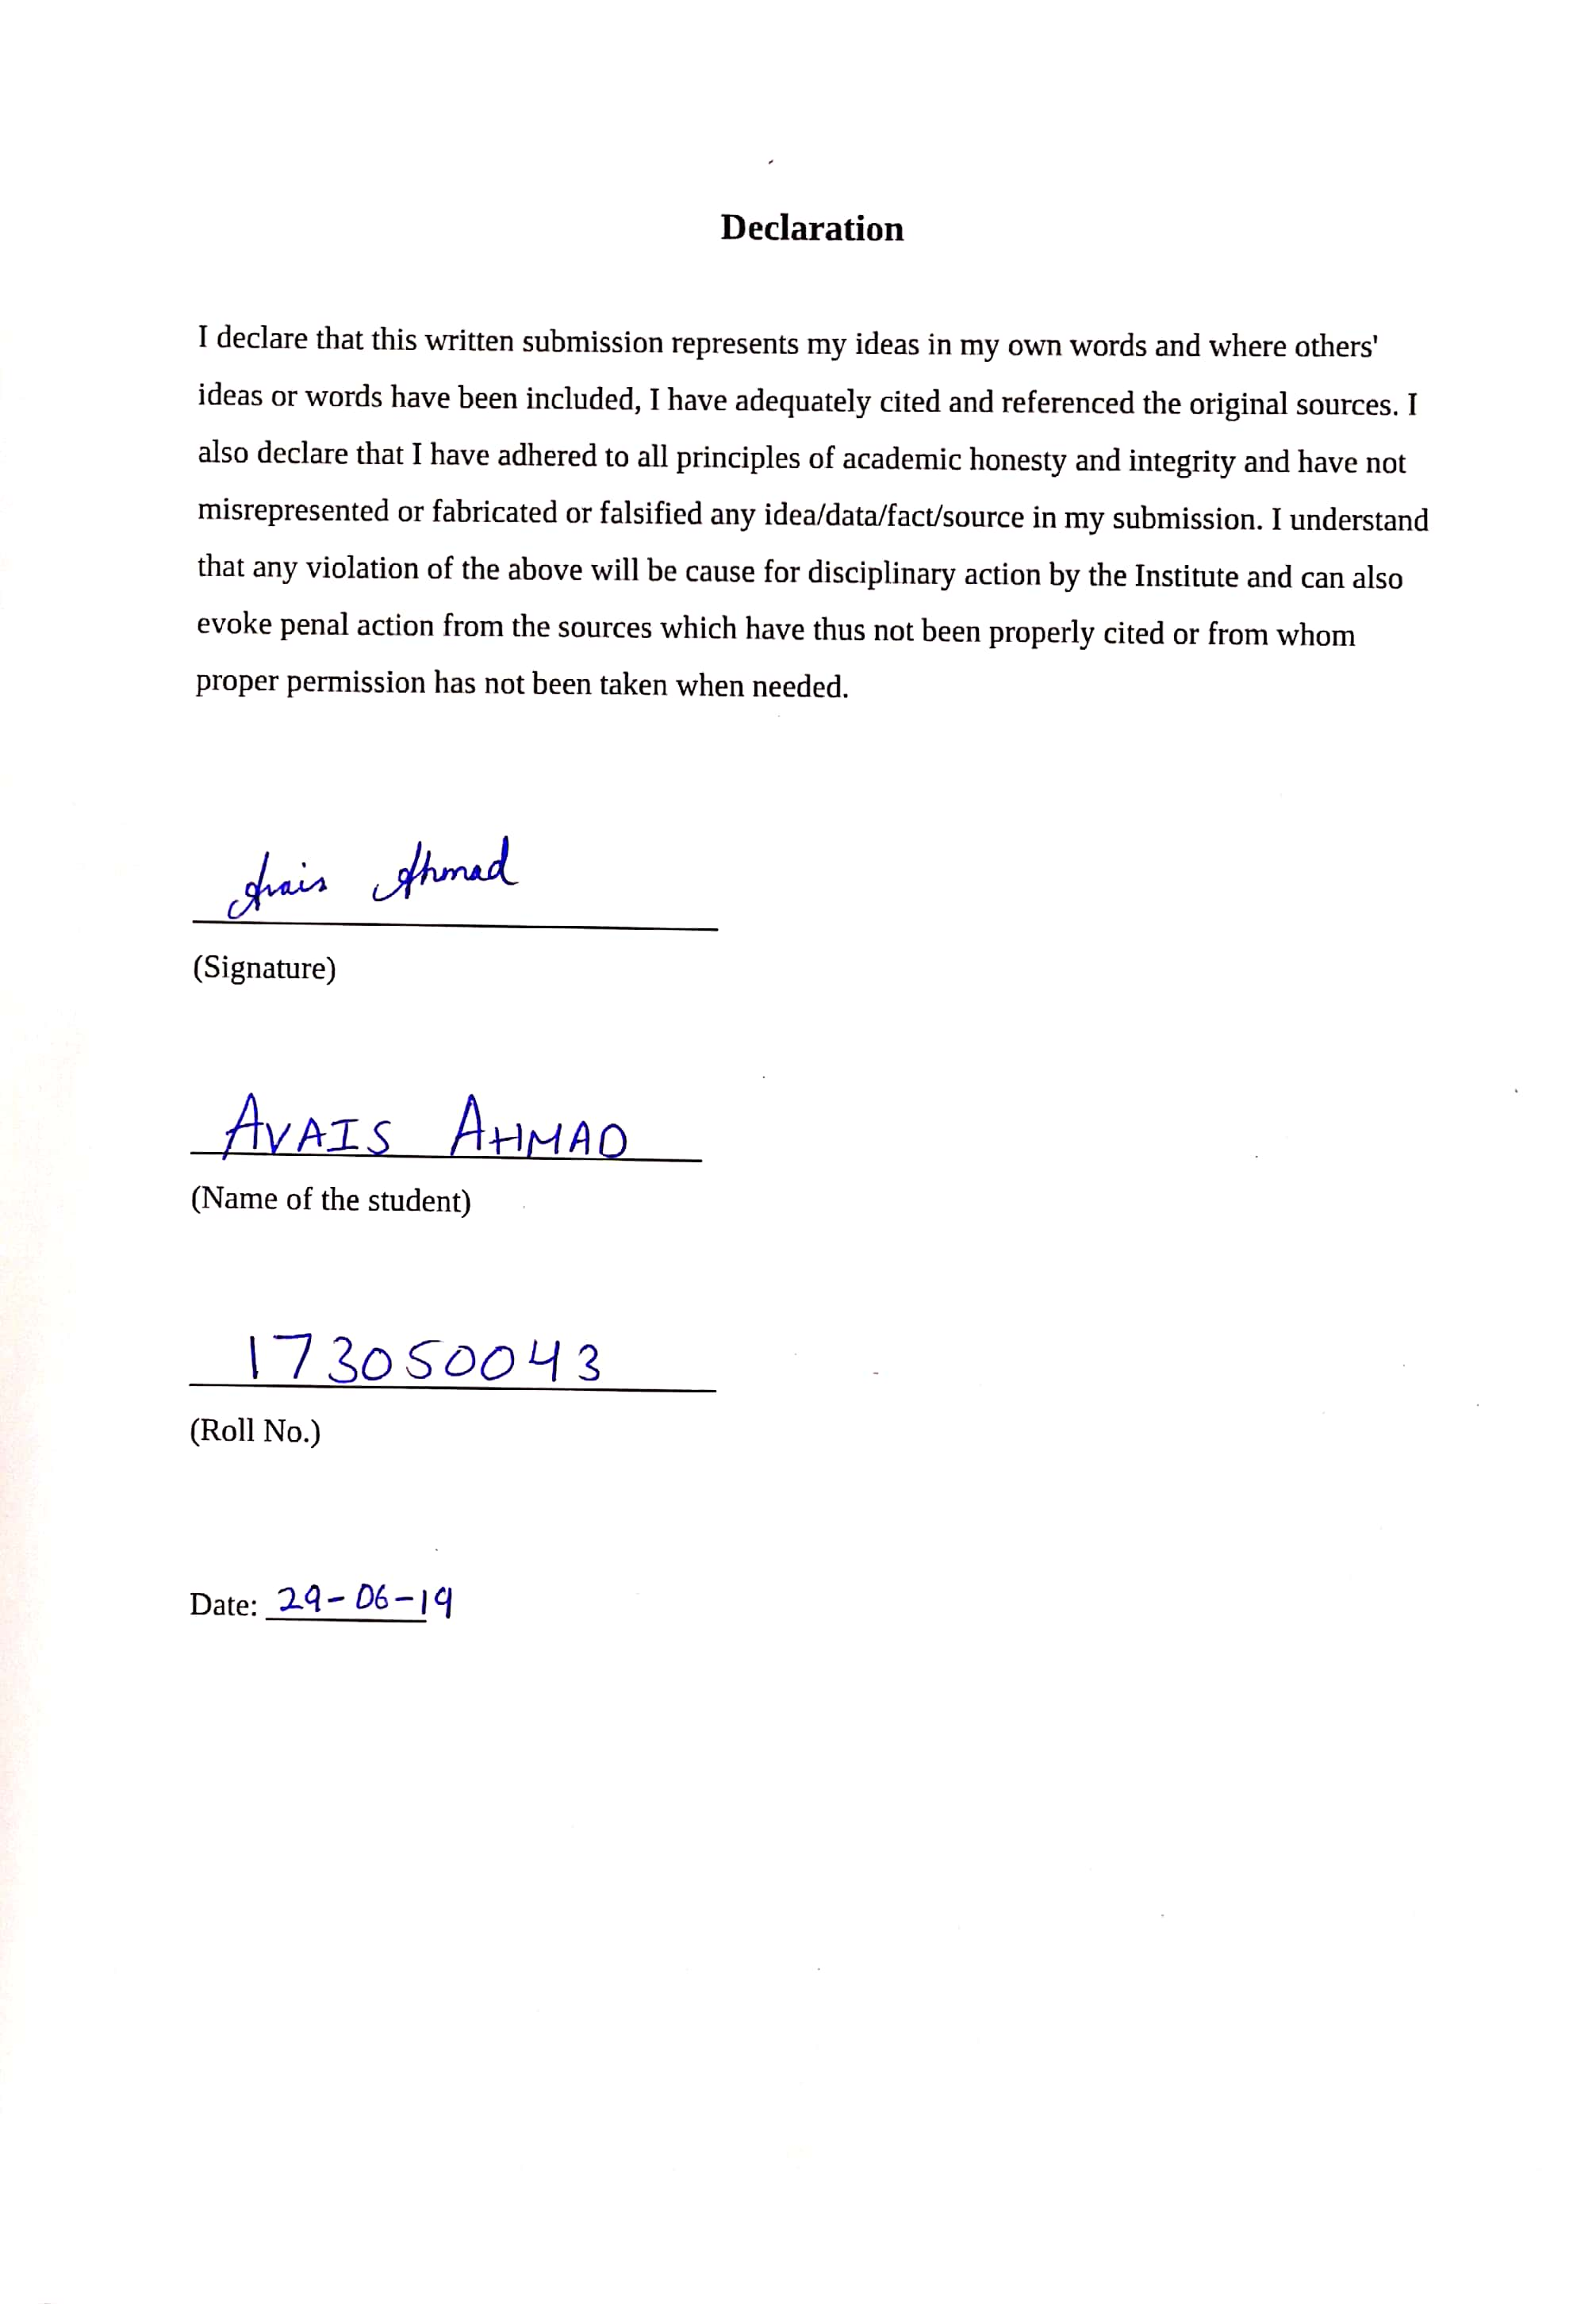
\includegraphics[width=\linewidth]{dissertation1.jpg}
\end{figure}


\section*{Acknowledgments}
I would like to thank \textbf{Prof. Paritosh K. Pandya} and \textbf{Prof. Kavi Arya} for their keen guidance and constant support. All the meetings and discussions were highly useful in understanding the basics. I would like to thank my parents for constantly supporting me in every facet of my life. I would also like to thank \textbf{Naveen Cherupally}  for helping me understand the basics of the problem \newpage

\thispagestyle{empty}
\section*{Abstract}
This thesis addresses High Level Programming of Embedded Systems such as Robots. Reliability of embedded systems are of matter of great importance. To be efficiently able to coordinate complex systems there are three techniques available: Synchronous Programming, Asynchronous Programming and Time Triggered Programming. Synchronous languages like Statechart, Lustre and Heptagon, Asynchronous languages like Linda and Time Triggered language like Giotto are available. This report contains their literature survey and how they can be useful for coordination. We combined the synchronous programming of Heptagon \cite{heptagon} with Time Triggered Programming inspired by Giotto \cite{giotto}. We call the resulting language as TTProg[Heptagon]. We have built a multi phase compiler for this high-level programming language and C-code is generated for final schedule. The automated compiler generate a static schedule which does not require any RTOS or context switching and is very useful for tight applications.

\tableofcontents
\newpage
\listoffigures

\newpage

\pagenumbering{arabic}

\chapter{Introduction}
The idea of \textbf{synchronous dataflow programming} comes from synchronous circuits. They take synchronous circuits as an abstraction and each step of the  execution is equivalent to working of the circuit for one clock cycle. Program consists of several concurrent modules which communicate via signals. It is assumed that both computation and communication take negligible time. Theoretically, the results should be available instantaneously at each clock. \\
Synchronous programming language are best suited for reactive systems. Reactive systems are a class to system which interact with environment continuously interact with the environment according to the speed imposed by the environment.


\begin{figure}[H]
\centering
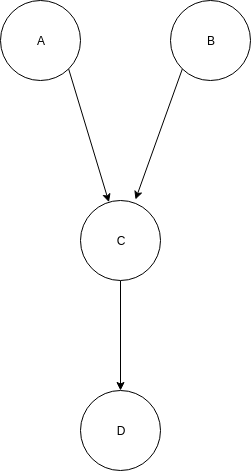
\includegraphics[width=0.25\linewidth]{fig5.png}
\caption{General idea of Synchronous Data flow language}
\end{figure}

In synchronous dataflow language order of the operations are not important. An operation can only fire if the result of its preceding dependencies are available. In the above figure node C can only fire if the result of A and B are available. So in declarative programming languages only the logic is defined and control flow is not important. \\
\noindent
According to \textbf{Synchrony Hypothesis}:
\begin{itemize}
    \item All the computation takes negligible time
    \item Communication takes negligible time
\end{itemize}
So we can assume that all the results are available instantly. This concurrency is logical. This style is good for complex control with concurrency.

In \textbf{Time Triggered programs} tasks are deterministically(periodically) triggered at specified time points. There may be data dependency between task computations. These computations may be time intensive, i.e. they take time. \textbf{Static Scheduling} is an attractive method of its implementation.

\textbf{Asynchronous programming} are much more powerful than synchronous programming languages. It allows parallelism and operations can run concurrently. Asynchronous programming make use of a several threads executing asynchronously to execute concurrent task. Once a task have completed its execution, it will update the result back to main thread. It will reduce waiting time of the overall process. We may also refer it as Parallel programming. For its implementation RTOS with context switching and memory allocation is needed.\\
It is helpful when we need to implement a distributed system. Suppose, there are some task which require to make use of database or require result by means on communication from some other module, they may require considerable amount of time to get result. It may delay the further execution of main thread. In asynchronous programming we may start them as the concurrent process and main thread will continue its execution. \\ 




\begin{figure}[H]
\centering
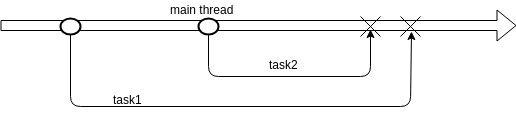
\includegraphics[width=\linewidth]{fig10.png}
\caption{Asynchronous Programming}
\end{figure}

In the above figure main thread invokes task1 and task2 which runs concurrently and communicates back the result back to main thread.


\textbf{Component Based programming} helps in designing the system with help of reusable components. Each functionality is separated in form of components. Each components are self contained with all the memory and functions needed. These components can be reused and can communicate with each other. It simplifies the designing of large complex systems.\\
In this report we will see how component based on synchronous and time triggered programming language are useful in designing complex systems.
We use an existing synchronous dataflow language Heptagon to program components with complex control flow. Alternatively, components may be programmed in C. Data intensive computations are implemented as C functions. \\
We then use a Time Triggered Programming Language Giotto to combine and coordinate the activities of components. This allows components whose steps of execution take time. \\
The components are combined in a deterministic fashion. The components may have data dependencies. The resulting language is called \textbf{TTProg[Heptagon] or TTHept} for short. As our main contribution, we propose a static scheduling based approach to implement the TTHept programs. The scheduling constraints due to data dependencies and computational requirements of components are derived and given to a constraint solver. \\
The resulting schedule is \textbf{statically} implemented as a sequential C program which does not require any RTOS or dynamic memory allocation. A prototype \textbf{compiler} is developed implementing the above technique.
A small case study on the Firebird robot illustrates our approach.


\chapter{Literature Survey on Synchronous programming Languages}


\section{Introduction to Statechart}

Statecharts are a form of visual programming language which provides the features like hierarchy, concurrency and communication. It is a synchronous language which is helpful programming reactive system. It is combination of a set of states and a set of transitions. We can broadly define statecharts as :-
\begin{equation}
    statecharts = state\_diagrams + depth + orthogonality +broadcast\_communication
\end{equation}{}

\begin{figure}[H]
\centering
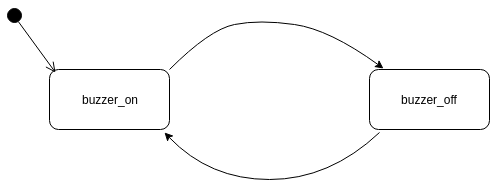
\includegraphics[width=0.85\linewidth]{fig1.png}
\caption{A simple statechart}
\end{figure}

\subsection{Clustering and Refinement}
Clustering means combining several states into a superstate. The sub states may share a common property for incoming or outgoing transitions. We can see an abstract model of the system by seeing the super state or we can zoom in , which can be 



\begin{figure}[H]
\centering
\begin{minipage}{.5\textwidth}
  \centering
  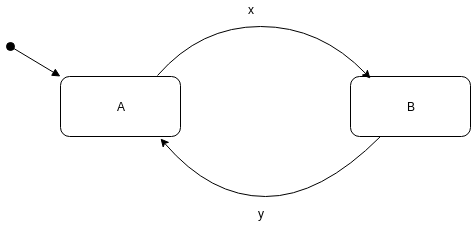
\includegraphics[width=\linewidth]{fig2.png}
  \caption{Clustering}
  \label{fig:test1}
\end{minipage}%
\begin{minipage}{.5\textwidth}
  \centering
  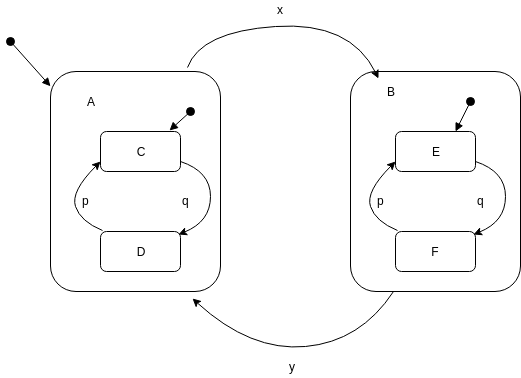
\includegraphics[width=\linewidth]{fig3.png}
  \caption{Refinement}
  \label{fig:test2}
\end{minipage}
\end{figure}

As shown in the above figure states C and D can be clustered into state A and states E and F can be clustered into state B. A common transition 'x' on state C or state D go to super state B. Similarly, a common transition 'y' will take state E and F to state A.


\subsection{Orthogonality}
An orthogonal state is AND of two or more states. In general transition system number of states can drastically grow due to AND composition. Orthogonal states simplifies this by running both the AND components concurrently.

\begin{figure}[H]
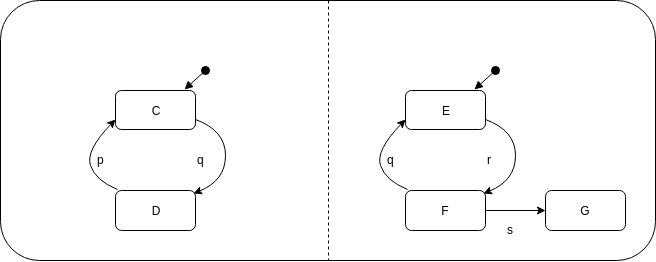
\includegraphics[width=\linewidth]{fig4.png}
\caption{Orthogonal State}
\end{figure}

The above orthogonal state will work same as product of those two sub states. Both sub states will execute concurrently. On the transition 'q' state C will jump to D and state E will jump to F.
On doing the AND product of them, the resultant state chart will contain 6 states.


\subsection{Broadcasting}
The components of state chart can communicate with each other by means of broadcasting. The broadcast values can be defined over transitions which can then be received by other components. This communication can be made deterministic by defining the order of execution.

\subsection{Yakindu Tool}
Yakindu is a statechart tool which can help in development of reactive systems. It provide a drag and drop interface for easy development of state charts. The execution of the statechart can be simulated. It provides a compiler which converts the statechart into C code. The functions definition can be then provided for each function which was defined on states or transitions. Following file are generated as the output of yaakindu tool:-
\begin{itemize}
    \item $<sc types.h>$: It is the header file that defines all the data types used.
    \item $<name>$.c : It contains the main execution of the statechart.
    \item $<name>$.h : It contains the variables, structures and fuction definitions required by .c file.
    \item $<name>$Required.h : This file expects the function definition from the user. It acts as the driver.
\end{itemize}{}

The typical program execution consist of three parts :-
\begin{itemize}
    \item init() :- It initializes value of all variables
    \item enter() :- It takes the execution to default state as the starting state
    \item runCycle() :- One execution of runCycle() is exuivalent to one step in statechart.
\end{itemize}{}


\newpage

\section{Introduction to Lustre}
Lustre is a synchronous programming language which is useful in designing reactive systems. It is a declarative language i.e. its execution consist of a set of equations. It make use of nodes as a unit if computation and data flow between the nodes. A simple example of Lustre node is:-

\begin{verbatim}

    node Sum(x,y:int)
    returns (S:int);
    let
        S= x+ y;
    tel
\end{verbatim}{}

\noindent
Above node will take two inputs as $x$ and $y$ and output's $S$ as their sum as S.\\

The programs in lustre is treated as a bunch of equations. At each cycle the compiler will solve them in a dependency order and produce output. Lustre does not allow  combinational loop. It neither allows syntactic nor semantic loop.

\subsection{Operations}
Following are some of the operations available in lustre:-
\subsubsection{if operation}
It is  used to assign value to a variable. In lustre if..then..else statement is not us as a program flow control statement but instead it is used to assign value to a variable. Example:-
\begin{verbatim}
    x = if y=5 then 1 else if y=0 then 2 else 0;
\end{verbatim}


\subsubsection{pre operation}
It returns the previous value of the evaluation of a statement. First pre invocation returns $nil$. It can be formally defined as:-\\ 
{
\centering

    For $(pre X)_i$\\
    if $i=0$ then undefined \\
    else $X_{i-1}$
    
}
\subsubsection{$->$ operation}
This operation is used to set initial value to a variable.It can be formally defined as  :-\\
$(X->Y)_i$, if i= 0 then X,else Y.\\
Example:-
\begin{verbatim}
    x= 0 -> y
\end{verbatim}
In the first execution, value of x will be 0 after that it will be same as y.

\subsection{Code Structure}
Lustre programs can be compiled and C code can be generated using $lv6$ (lustre v6) command. Following are important C files are generated as output:-
\begin{itemize}
    \item lustre\_types.h : It contains definition of various data types used in the C code.
    \item $<filename>$\_$<nodename>$.h : It contains the function definition for the functions which are used in its C file
    \item $<filename>$\_$<nodename>$.c : It basically contains step and reset function of all the nodes involved. The reset functions initialize the value of variables and step function is equivalent to one run cycle of the program.
    \item $<filename>$\_$<nodename>$\_loop.c : It contains the main function and a infinite while loop in which step function of the node is indefinitely invoked.
\end{itemize}

\newpage

\section{Introduction to Heptagon}
Heptagon \cite{heptagon} is also a synchronous data flow language which is inspired by lustre. Its syntax and semantics are mostly common with lustre. Similar to lustre it also use nodes as an unit of data flow. It take input and produce output as a sequence. \\

\subsection{New operations}
Operators like if , pre and $->$ (initialization) are same as that in lustre. Heptagon provides various control structures which were not previously present in Lustre.

\subsubsection{Switch}
It helps in controlling how the program flows based on given condition. The condition in the switch statement can be either Boolean or enumerated. Example of switch:-
\begin{verbatim}
node bin(x:bool) returns (y:int);
let 
    	switch x
    	| true do y=10 
    	| false do y=20 
    	end
tel
\end{verbatim}

In the above example the value of output y will be 10 if x is true otherwise 20.

\subsubsection{Present}
Present is similar to switch. It allows multiple expression to be evaluated in a single step. To make the execution deterministic the expressions are evaluated sequentially. \textbf{last} keyword use the memory which is shared by different modes.\\
Example of present control structure:-

\newpage

\begin{verbatim}

node bin(x:int) returns (y:int)
var last p:int =0;
let 
    	present
    	| x>5 do p=10 
    	| x>10 do p=20
    	| x<=5 do p=30 
    	end;
    	y=p

tel
\end{verbatim}
In the above example the value of output y will be 10 if x is greater than 5 and less than 10, 20 if x i greater than 10 , 30 otherwise.

\subsubsection{Automata}
Automata is one of most powerful function provided by heptagon. Automata is a transition system which consist of a set of states and a set of transitions. At a given time automata can be present at any one of the states. The current state determines which set of instructions the node will execute. The transitions are invoked by a given set of condition. Heptagon provides two clauses for invoking the transitions of the automata:-
\begin{itemize}
    \item until e then S : It is used to define weak transitions. In this state when the expression e becomes true the target state S is executed in the next instance.
    \item unless e then S : It is used to define strong transitions. In this state when the condition becomes true the target state S is executed in the same instance.
\end{itemize}{}

\begin{figure}[H]
\centering
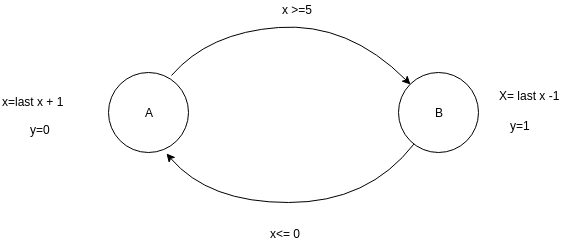
\includegraphics[width=\linewidth]{fig6.png}
\caption{Automata Example}
\end{figure}


The above automata can be simulated using heptagon as follows:-
\begin{verbatim}
node atm() returns(z,y:int)
var last x: int =0;
let
    y=x;	
    automaton
        state A
            do x= last x +1; z=0
            until x>=5 then B
        state B
            do x= last x -1;z=1
            until x<=0 then A
    end
tel
\end{verbatim}{}





\subsubsection{Array}
Array are the collection of similar data types. Arrays are declared in heptagon by using \^{} operator.
Followig is the syntax for array:-
\begin{itemize}
    \item \textbf{Declaration}:- $<datatype>$\^{}$<size>$
    \item \textbf{Multidimensional}:- $<datatype>$\^{}$<size>$\^{}$<size>$.Example, int\^{}m\^{}n is interpreted as (int\^{}m)\^{}n.
    \item \textbf{Accessing}:- Array elements can be simply accessed as name[constant\_index]. Dynamic index are indexed as out = name.[index]
    \item \textbf{Extracting}:-  A slice of array can be extracted from already existing as old[s..e]. The new array will contain all the elements starting from s to e.
\end{itemize}{}
Operations on array can be performed using iterators which are discussed ahead.

\subsubsection{map}
Map is an iterator using which we can apply a node to arrays to produce another array as output. Syntax for map operator is :-\\
map $<<n>>$ node (a1,a2)\\
Here n is the number of elements. $node$ refers to the node which will be invoked as an unit function and a1,a2 are the input array.
Example:-
\begin{verbatim}
node ss (a,b: int) returns (c:int)
let
     c = a+b;
tel

node mapSum (t1,t2: int^5) returns (out: int^5)
let
    out = map <<5>>ss(t1,t2);
tel
\end{verbatim}

Above example will produce sum of t1 and t2 as output. mapi is a variation of map which implicitly provides a iteration index.
  


\subsubsection{fold}
Fold is an iterator using which we can apply node to array to produce a scalar output. Syntax of fold operator is :-\\
fold $<<n>>$ node (a1,a2,i)\\
Here n is the number of elements. $node$ refers to the node which will be invoked as an unit function and a1,a2 are the input array. i is the variable into which the operations will be performed to produce output.
Example:-

\begin{verbatim}
node addn(a,x,y: int) returns (z: int)
let
    z = a + x * y ;
tel

node foldAdd(x,y: int^3) returns (z: int)
let
    z = fold  <<3>>  addn (x,y,0);
tel
\end{verbatim}
Above example will produce scalar product of all the elements of the array x and y.Similar to mapi , foldi also implicitly provides a iteration index.



\subsubsection{mapfold}
Mapfold is an iterator which is a combination of map and fold. It can be used to get scalar value as well as an array in the output. Syntax of mapfold is :-\\
mapfold $<<n>>$ node (a1,a2,i)\\
Here n is the number of elements. $node$ refers to the node which will be invoked as an unit function and a1,a2 are the input array. i is the variable into which the operations will be performed to produce output.


\subsubsection{Interfaces}
Interfaces are only declaration without and definition for node , function or types. They are put into .epi files. The definition for the interface can be provided externally. To use the interface inside our Heptagon code we have to open the file.epi file as follows:-\\
open File

\subsection{Code Structure}
Command for compiling a heptagon file and generating a C code is\\
{

\centering
heptc -target c file\_name.ept

}
Important files generated as output are:-
\begin{itemize}
    \item $<name>$.h: This header file contain a structures for storing the output and intermediate computation of the the node, they are suffixed as out and mem respectively. It also contains the declaration of the step and reset functions for the nodes.
    \item $<name>$.c: This file contains the definition for the reset and step function. The reset function initializes the values of the variables. The step function do the intermediate computations and updates the value of of the structures which were present in the header file.
\end{itemize}{}

\subsection{Heptagon Example}
In the following examples heptagon is used as a coordinator for Firebird V robot. Firebird V works on Atmega 2560 microprocessor. To be able to use heptagon on the robot special module of code (Input/Output drivers) are used. 



\begin{figure}[H]
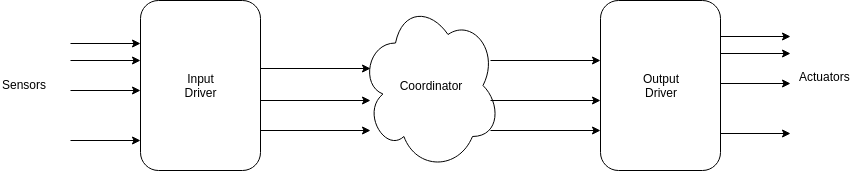
\includegraphics[width=\linewidth]{fig7.png}
\caption{Using heptagon as a coordinator}
\end{figure}

Input driver takes inputs from various sensors and convert it into logical and simplified form so that it could be passed to heptagon. Output driver takes the logical output from heptagon and convert it into actual values and invoke the actuators using that value.\\
One cycle of the program will contain following steps:-
\begin{itemize}
    \item Reading values from the sensors
    \item Converting those values into a logical form and passing it to heptagon coordinator
    \item Applying the heptagon coordination logic and generating the output
    \item Converting logical output into actual output
    \item Invoking actuators using the output  generated.
\end{itemize}{}


\subsubsection{Adaptive Cruise Control}

In this example firebird V will robot will keep  following the white line unless it detects an obstacle. If the obstacle is near it will slow down, if the obstacle is very near it will  stop.

\begin{figure}[H]
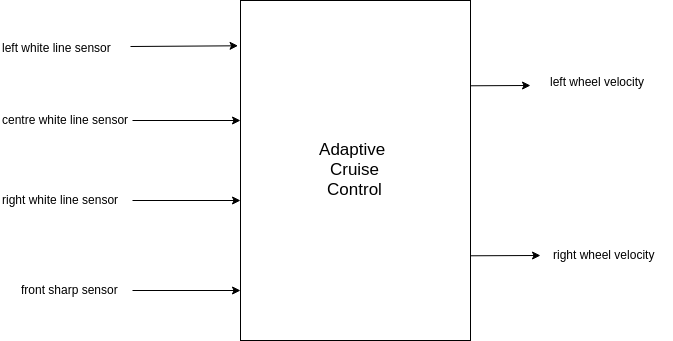
\includegraphics[width=\linewidth]{fig9.png}
\caption{Adaptive Cruise control as a Black Box}
\end{figure}

The logical conversion done by input driver are:-
\begin{itemize}
    \item \textbf{distance} : It is determined based on value of Front Sharp Sensor.
            \begin{itemize}
                \item (Sensor value $>$ 150 ) :means obstacle is far , distance value will be set to 0
                \item (Sensor value $>$ 40 and $<$ 150 ) :means obstacle is near , distance value will be set to 1
                \item (Sensor value $<$ 40 ) :means obstacle is very near , distance value will be set to 2
            \end{itemize}
            
    \item \textbf{leftOut,centreOut and rightOut} : If their respective sensor value is $>0x40$ it will be set to 1 otherwise 0
\end{itemize}

The conversion done by output driver are of setting speed of the wheels. These mappings can be changes according to the need. The speed of wheels are divided into five range :-
\begin{itemize}
    \item Logical 0 = Actual 0
    \item Logical 1 = Actual 50
    \item Logical 2 = Actual 130
    \item Logical 3 = Actual 150
\end{itemize}



\noindent
Following is the coordinator code written in heptagon:-


\begin{verbatim}
node distanceToSpeed (distance: int ) returns (speed :int);
let
    speed=if distance=2 then 3
          else if distance=1 then 2
          else 0;
tel


node acc(distance : int; leftOut,rightOut,centreOut : bool)
returns (wheelLeft,wheelRight : int);
let
    wheelLeft= if(centreOut = false) then distanceToSpeed(distance)
            else if(centreOut = true and leftOut =true and rightOut=true) then 0
            else if leftOut=true then 2
            else if rightOut=true then 1  else 0;

    wheelRight=if(centreOut = false) then distanceToSpeed(distance)
            else if(centreOut = true and leftOut =true and rightOut=true) then 0
            else if leftOut=true then 1
            else if rightOut=true then 2  else 0;
tel
\end{verbatim}{}


\section{Asynchronous Programming and Linda}
Linda is an asynchronous coordination language. It was developed at Yale University. It gives a model of concurrent programming and parallel processing. It makes use of tuple space trough which processes can communicate.A linda program can be seen as combination of distributed coordination and sequential computation. Linda can be used along with many languages such as C, Java ,Prolog etc.

\begin{figure}[H]
\centering
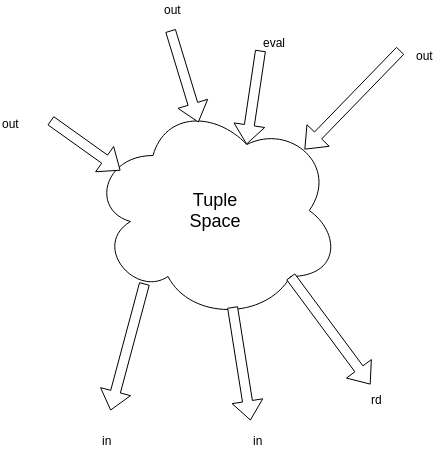
\includegraphics[width=0.8\linewidth]{fig8.png}
\caption{Tuple Space}
\end{figure}
The tuple space acts as a shared memory in which processes can get or put data. Once a tuple is added into tuple space ir is expected to stay until some other process explicitly removes it. Two types of tuples present in the tuple space are live tuple and data tuple. Live tuple are process under evaluation while data tuple are stored form of data. \\
\subsection{Operations}
Various operations of linda are:-
\begin{itemize}
    \item \textbf{out}: This operation is used to put a tuple into tuple space.
    \item \textbf{in}: This operation try to match the tuple in tuple space, if the match is found the tuple is read and it is removed from the tuple space.
    \item \textbf{rd}: It is similar to in operation. Only difference is that tuple remains in the tuple space even if the match is found.
    \item \textbf{eval}: It crates a live tuple or process in the tuple space and the expression is evaluated after being added.
\end{itemize}

\subsection{C-Linda program structure}
A typical C-Linda program can be compiled using "clc -o out name.cl" , where .cl is file which contains a C-Linda program and out is the executable file.
General structure of the program is as follows:-
\begin{verbatim}
int main()
{
    //genera1 c instructions
    
    //staring a process in tuplespace for some computation
    eval("slave1", x , fun(x));
    
    
    //reading "result" tag from the tuple space
    rd("result" ,? var2);
}

int fun(int x)
{
    //some computations
    
    out("result", var1);
}

\end{verbatim}{}


In the above program a process with the tag slave1 is started to do some computation. When "slave1" is done with computation it will update the output of var1(some variable) with the "result" tag into the tuple space. Once the output is updated with the tag ""result" , its value can be read and stored in variable var2.

\section{GALS model}
Globally asynchronous locally synchronous is a modal in which we divide the system into several synchronous components. It can be seen as network of reactive components, each component will execute with its own clock. These components can communicate with each other asynchronously.\\
This model can be very useful for designing large complex systems as it will provide much higher level of abstraction. Using a asynchronous layer at the top of synchronous programming language will help in as it will reduce the number of possible states in the system.\\
We generally require Real Time operating systems to implement GALS model.


\chapter{TTProg: Time Triggered Programming}


\section{Giotto Inspired TTProg}
Giotto \cite{giotto} is a time triggered programming language which provides a programming environment using which we can program embedded systems. It is useful in designing the systems with hard real time constraints. Giotto provides semantics by which we can easily model systems which are periodic and systems with multiple modes. \\
A control design is first converted into a Giotto program which is then converted into code for real time platform by means of hardware mapping and scheduling. \\
We will be building a Time Triggered Program(TTProg) which is a simplified version of Giotto. In this simplified version we will be only working on a single mode so complexity of mode switching is eliminated. Also, we are not using guards for drivers in this implementation.\\
Key advantages of this are that task are triggered at fixed(periodic) times. Task are preceded by drivers which communicate data at fixed time resulting in deterministic execution.
Three main elements of a TTProg program are :- 
\begin{itemize}
    \item \textbf{task} : They are the main functional unit of a TTProg 
    \item \textbf{driver} : They act as mode of communication between sensor, actuators and tasks.
\end{itemize}{}

\section{Definition of TTProg}

\subsection{Ports}

Ports are the memory by which data communication happens in TTProg.
Ports can be defined as (p,Type,init):-
\begin{itemize}
    \item \textbf{p} : it is the name of the port
    \item \textbf{Type} : it is the type of the port
    \item \textbf{inti} : it is the initial value of the port , $ init \in Type$
\end{itemize}
  
Ports name should be unique. A port can be either of sensor port, actuator port or private port.


\subsection{Tasks}
Functionalists in TTProg are performed by means of tasks. 
Tasks can be defined as (t,In,Out,Priv,f):-
\begin{itemize}
    \item \textbf{t} : it is the name of the task
    \item \textbf{In} : it is the set of input ports
    \item \textbf{Out} : it is the set of output ports
    \item \textbf{f} : it is the function which the task performs. $f: Value[In \cup Priv] \rightarrow  Value[Out \cup Priv]$
\end{itemize}
It can be seen as encapsulation of ports and a functionality. Two tasks cannot share input and private ports , the can share output ports as long as they are not in same mode. A task frequency is defined which tells home many times  task needs to be invoked in total time period of the mode.

\subsection{Drivers}
Drivers are the atomic tasks which help in communication between tasks and between task with sensor and actuator.
Drivers can be defined as (d,Src,Dst,h):-
\begin{itemize}
    \item \textbf{t} : it is the name of the driver
    \item \textbf{Src} : it is set of source ports for the drivers
    \item \textbf{Dst} : it is the set for destination ports for the driver
    \item \textbf{h} : it is the function invoked by the driver
\end{itemize}
The function h will take the values of the source ports as inputs and maps it to the output port's value. They are atomic and are performed in logically 0 time.


\subsection{Task Invocation}
TTProg tasks are invoked at a regular interval which is decided by the frequent $\omega$ provided. The time of execution of task can be determined by dividing time period of the mode by $\omega$. Task invocation can be defined as ($\omega_{task}$,t,d) :-
\begin{itemize}
    \item \textbf{$\omega_{task}$} : it is the frequency for the task
    \item \textbf{t} : it is the name of the task
    \item \textbf{d} : it is the driver for the task
\end{itemize}{}
It include the communication phase and the execution  phase. At the end of task invocation the outputs are available at the output ports.


\section{Logical Execution}
\begin{figure}[H]
\centering
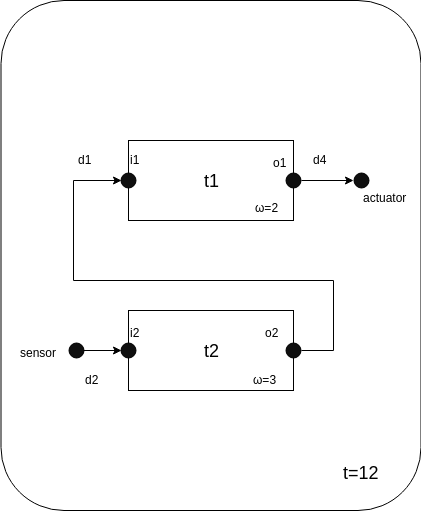
\includegraphics[width=0.6\linewidth]{24timingData.png}
\caption{Timing and Data Dependency Diagram}
\end{figure}

As we can see in above diagram there are two tasks t1 \& t2 running concurrently. Task t1 have input port i1 and output port o1. On other hand task t2 have input port i2 and output port o2. Driver d1 reads value from port o2 and assign value to i1. Driver d2 reads value from port o2 and assigns value to port i1. Driver d2 reads value from the sensor and assigns value to i2. Driver d4 reads value from o1 and do the actuation.
A driver must be assigned to provide input to any task. \\
Time period of the program is 12ms i.e. one cycle of execution takes 12ms. Frequency is t1 is 2 therefor it must execute two times in the cycle giving 6ms of logical time to one tasks instance. Similarly t2 must execute 2 time in the cycle giving 4ms logical time to each instance. The drivers are assumed to execute instantly.



\begin{figure}[H]
\centering
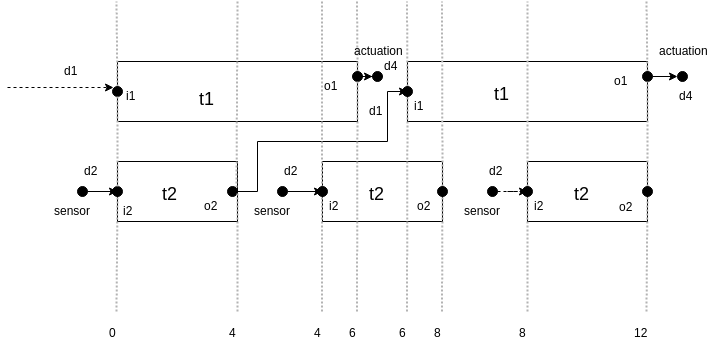
\includegraphics[width=0.9\linewidth]{10Example.png}
\caption{Timeline}
\end{figure}

The above \textbf{timeline} shows the unfolding of the above example. We can observe that $1^{st}$ instance of t1 is dependent on output produced by previous instance of t2. Second instance of t1 depends on output produced by the first instance of t2. The logical time given to each task is calculated by dividing time-period by frequency. This logical time give each task a start time and a end time. For example start time for $1^{st}$ instance of t1 is 0 and end time is 6 ms. The task execution must start after start time and end time. Even if the task finish its execution before end time the values of output port will be only available at is end time. Similarly, values of start port must be available at start time.

\section{Formal Semantics for TTProg}
For execution, Giotto specifies strict time for start time and end time for each task and drivers. These semantics are too strict and will prevent execution in practical scenarios. To to able to schedule these on real world systems we will need to convert this to an equivalent sequential schedule.


\subsection{Program Configurations}
Program Configurations defines the current state of the execution of the program. Logical execution of Giotto is strictly defined by these by these configuration. Program configuration is defined as:
\begin{equation}
    C = (m,\delta, v, \sigma_{active},\tau)
\end{equation}
\begin{itemize}
    \item \textbf{m} is the mode in which currently the program is. For our TTProg, we have only only single mode
    \item \textbf{$\delta$} is the mode time. For our TTProg it will start form 0 for every cycle of mode.
    \item \textbf{v} is the current valuation of the ports
    \item \textbf{$\sigma_{active}$} is the set of logically active task. It may or may not be running physically
    \item \textbf{$\tau$} is the time stamp of the program
\end{itemize}

\subsection{Micro Steps}
Each of the successor program configuration is a result of running the Micro Steps in the order. The time at which the configuration is updated is determined by the LCM of frequency of all the task and drivers. This LCM is then divided by the time period of the mode.\\
Let $T$ be the time period of the mode and $\omega_{LCM}$ be the LCM of frequencies, then configuration should update after every :
\begin{equation}
  C_{update} =  \frac{T}{\omega_{LCM}}
\end{equation}

Our Giotto inspired TTProg have reduced number of micro steps as mode switching is eliminated. 
\begin{figure}[H]
\centering
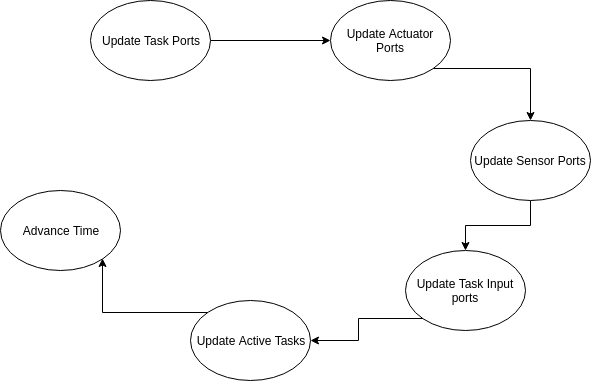
\includegraphics[width=\linewidth]{18microSteps.png}
\caption{Configuration}
\end{figure}

 \begin{itemize}
     \item \textbf{Update Task Output Ports :-}Output ports of previously completed task should be updated
     \item \textbf{Update Actuator Ports }Once the task port is updated the dependent actuator are updated next
     \item \textbf{Update Sensor Ports :-}Sensor read is performed and sensor port are updated next
     \item \textbf{Update Task Input Ports :-}Input port of the task are then initialized by its drivers
     \item \textbf{Update Active Task :-}No of task active are now updated
     \item \textbf{Advance time :-}Time at which micro steps should execute next should be updated
 \end{itemize}

We can also say that at every $C_{update}$ time program will go through series of micro steps and will apply whichever is applicable.

\subsection{Example}
Taking the instance of our previous example where the Mode period is 12 ms and the frequency for the task are 2 and 3. Therefore, the configuration will update after every 2 ms.
\begin{figure}[H]
\centering
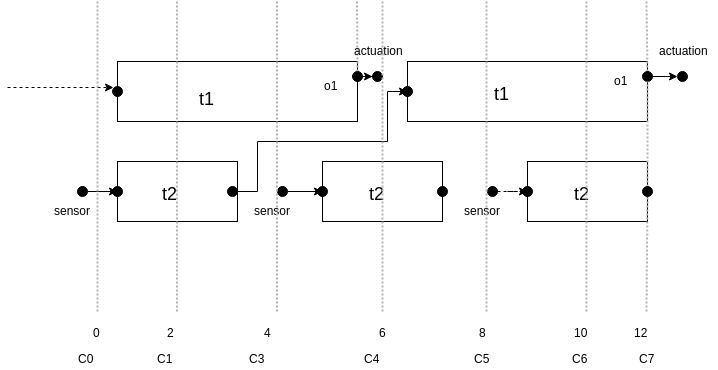
\includegraphics[width=\linewidth]{19config.png}
\caption{Configuration}
\end{figure}

As we can see in above diagram:-
\begin{itemize}
    \item $C_{0} $ Output port of previous execution will update, sensor will read and input port will be initialize. New active task will be t1 and t2
    \item $C_{2} $ noting will happen
    \item $C_{4} $ Output port of t2 update, sensor will read and input port of t2 will be initialize. Active task will remain t1 and t2
    \item $C_{6} $ Output port of t1 will update, actuator update will occur and input port of t1 will be initialize
    \item $C_{8} $ Output port of t2 update, sensor will read and input port of t2 will be initialize. Active task will remain t1 and t2
    \item $C_{10} $ noting will happen
    \item $C_{12} $ Output port of will update, and so on
    
\end{itemize}

\section{Compiler Implementation}
Using this TTProg we will first automatically map user provided task to Giotto like structure. After that we will find all the set of \textbf{constraints} to be followed to keep the flow of data(as ports) deterministic between tasks. These constraint will be generated based on worst case execution time(\textbf{wcet)} for each task. Once we have all the constraints we will require a constraints solver such as \textbf{Z3} to get the correct ordering and staring point for each task. We will eliminate this requirement to start all the task at specified time, only sensor and actuator update will be triggered at specific time and task dependent on them will be delayed. We will call this \textbf{time abstract schedule}, it will be free from wcet and it will keep data flow between ports deterministic. Once we have this schedule the final compiler will generate C code based on this schedule. This auto generated C-code will use timer based interrupts to deploy a set of schedule at specific time.

\begin{figure}[H]
\centering
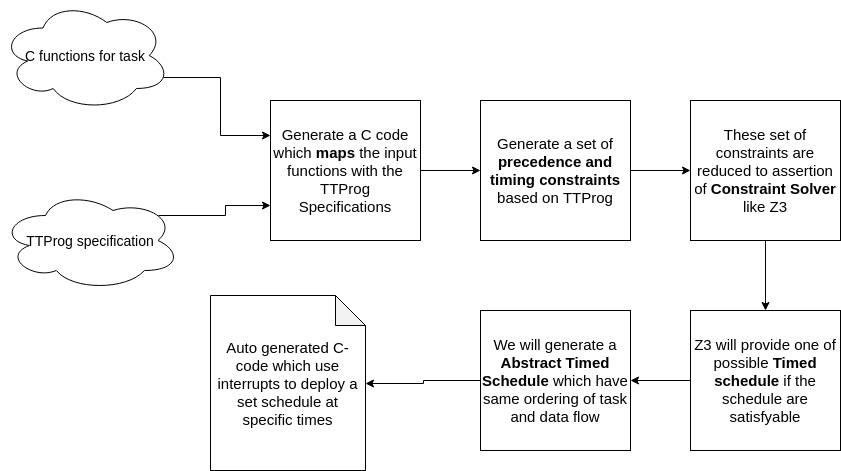
\includegraphics[width=\linewidth]{compiler.png}
\caption{Compiler Implementation}
\end{figure}

\section{Issues}
Following are the issues in practical scenario for these logical execution:-
\begin{itemize}
    \item Task are running concurrently in the logical execution, to mimic this kind of execution one may require multiple host or context switching
    \item The time required by the logical execution depends on the frequency of the and the mode period, actual execution of task may finish much before that.
    \item Logical execution assumes that the configuration updates instantly at logically 0 time. In real world this is not the case as micro steps requires a number of sensor read and actuator update which may require some amount of time 
    \item Task which are supposed to be executed at specific time like sensor read and actuator update will require some jitter tolerance.
\end{itemize}


\chapter{TTProg${[}$Heptagon${]} $ and Input Structure}



\section{Motivation}
Heptagon can be directly used to coordinate simple functionalities which are based on synchronous data flow and  don't require time intensive computations. Following are the reasons that motivates us to use a Time Triggered Asynchronous layer along with Heptagon:-
\begin{itemize}
    \item Heptagon is good for periodic task but it fails for time/computation intensive task as it assumes that the results are computed instantly
    \item Generating a \textbf{statics schedule} based on all the ordering and timing constraints for the task will give us bare metal implementation
    \item It will eliminate any requirement of RTOS
    \item No context switching is required so lot is overhead is eliminated
    \item The program will be deterministic and memory will be statically initialized
    \item It will give extreme speed to tight application
\end{itemize}


\section{TTProg${[}$Heptagon${]} $ Proposal}
The idea is to implement Giotto inspired TTProg on the top and inside it using heptagon for local synchronous components. Giotto contains modes within which there can be multiple tasks. Tasks are the functional unit of the Giotto program, they can a C code. These tasks run periodically and communicate with each other. These tasks can be replaces with an equivalent heptagon program. \\
Tasks are declared as (t,In,Out,Priv,f). We can see a similar structure in an heptagon node. 

\begin{figure}[H]
\centering
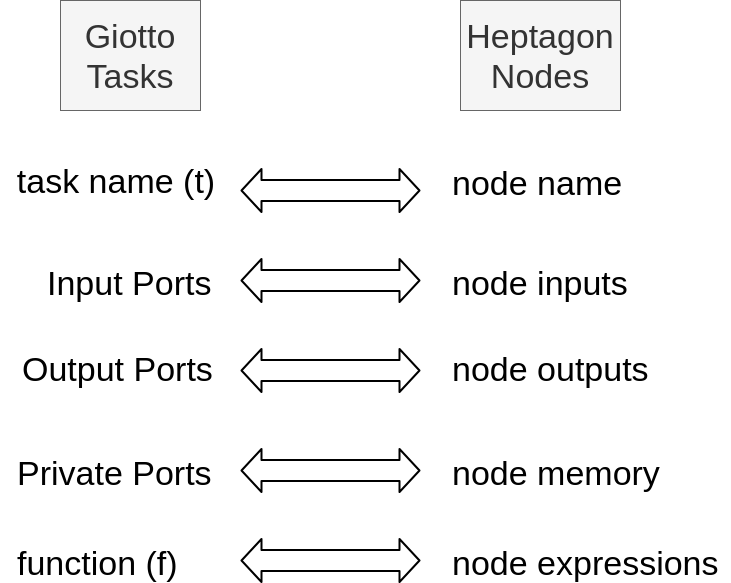
\includegraphics[width=0.9\linewidth]{fig12.png}
\caption{Task- Node mapping}
\end{figure}

As we can see in above figure, a Giotto task can be completely mapped to a heptagon node.
\begin{itemize}
   \item \textbf{t} which is the task name is same as name of the heptagon node
    \item \textbf{In} which is the set of input ports is same is the inputs which are passed into heptagon node.
    \item \textbf{Out} which is the set of output ports is same as the output produced by a heptagon node. It is internally stored in the form of C structure.
    \item \textbf{Priv} which is the set of private ports is same as the memory used in heptagon node while performing operations like pre. It is also internally stored in the form of C structure.
    \item \textbf{f} which is the function which the task performs. $f: Value[In \cup Priv] \rightarrow  Value[Out \cup Priv]$ can be seen as the bunch of equations a heptagon node performs in order to perform certain logic.
\end{itemize}{}

Complete mapping can be done by adding a layer of driver between ports and heptagon. 




% \begin{z3}

% linear formulas


% \section{Example}
% To demonstrate the idea let us take an example of pick placer theme. It consist of a grid Arena with designated pick up and drop points. The robot have to traverse thought the black line of the grid to pick up blocks and then drop them on the designated points.


% \begin{figure}[H]
% 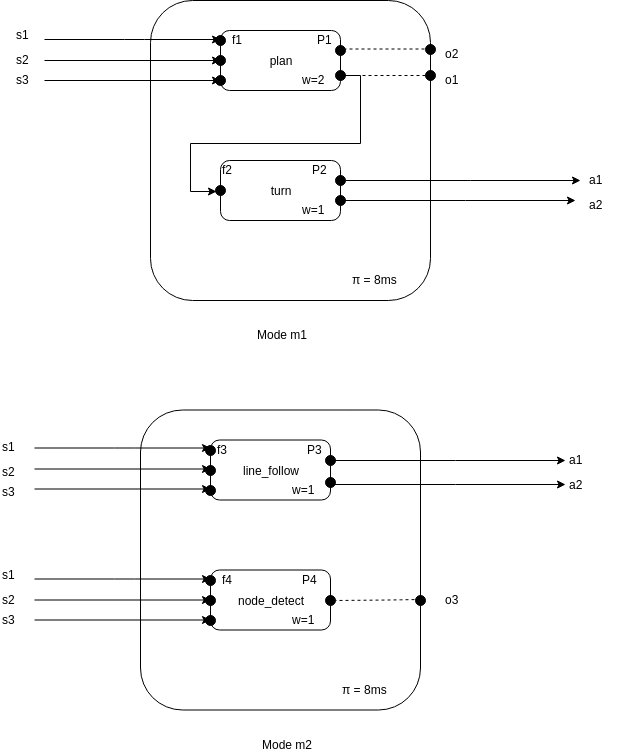
\includegraphics[width=\linewidth]{fig13.png}
% \caption{Pick placer using Giotto[Heptagon]}
% \end{figure}

% In this example the action of picking up and dropping the box is skipped. Only the action of planning and following the path is considered. All the tasks are heptagon program.\\
% The example consist of two modes m1 and m2. In the mode m1 there are two tasks "plan" and "turn". The plan heptagon node will take the value of all three white line sensor as input. They will be processed by means of some drivers. It will produce two output ports o1 and o2. o1 will let the "turn function know, which direction to turn. It can be either clockwise, anticlockwise or no turn,  hence 3 values. The turn function will send the actuator update a1 and a2. a1 will be the velocity of left wheel and s will be the velocity of right wheel.\\
% Output o2 will act as a guard for mode switch to m2. When the robot have turned to correct direction it will switch to mode m2 t start following the line. \\
% As private ports it will store the information of coordinates and current direction.
% Whenever plan task is invoked it will first update its coordinates and then it will decide which direction to turn the robot.\\

% The m2 consist of two tasks "line\_follow"  and "node\_detect". Both of them takes values of all three white line sensor as input. The task line\_follow will generate two outputs a1 and a2 as actuator update. a1 will be the velocity of left wheel and s will be the velocity of right wheel.The task node\_detect will generate o3 as output which is the guard for mode switch to m1. Whenever a node is detected it will switch back to mode m1.



\section{Input Structure}
The TTProg compiler requires a C header file which contain the functions for Task and Drivers. These functions can be either generated using Heptagon or could be manually written. Apart from this header file we need to also provide a TTProg program which is written as a JSON object. 


\begin{figure}[H]
\centering
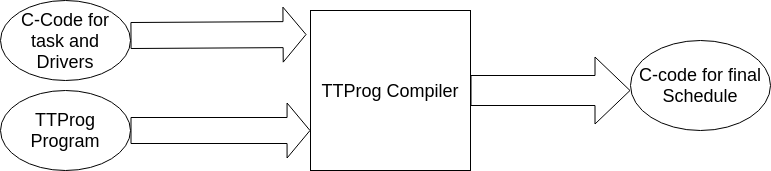
\includegraphics[width=0.9\linewidth]{9GiottoStructure.png}
\caption{TTProg Structure}
\end{figure}


TTProg compiler will compile in multiple phase and generate final C-code for a satisfying schedule.

\subsection{giotto.json input file}
JSON format makes it very easy to write and parse the TTProg program. As whole program is already present as an object we can simply read the file and refer required fields. This approach also reduce the chances of error as we only need to keep in mind the JSON and Giotto syntax.\\
Let us consider the following of logical execution of a instance of TTProg.

\begin{figure}[H]
\centering
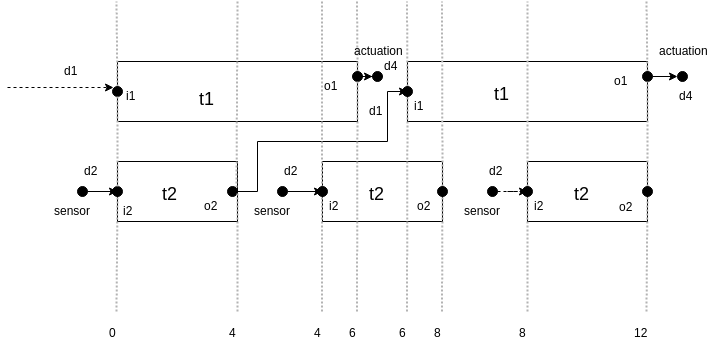
\includegraphics[width=0.9\linewidth]{10Example.png}
\caption{Sample Example}
\end{figure}

The above logical execution have two instance of task t1 and 3 instance of task t2. Each task is associated with some ports and drivers. giotto.json program for the above example will be :-
 \begin{verbatim}
     {
    "sensor" : [
        {"name" : "s1" , "type" : "float"}
    ],

    "actuator" : [
        {"name" : "a" , "type" : "float" , "init" : "0"}
    ],
    
    "input" : [
            {"name" : "i1" , "type" : "float"},
            {"name" : "i2" , "type" : "float"}
    ],

    "output" : [
        {"name" : "o1", "type" : "float" , "init": "0"},
        {"name" : "o2", "type" : "float" , "init": "0"}
    ],

    "task" : [
        {"name" : "t1", "input" : ["i1"] , "output": ["o1"], 
        "function":"f1", "wcet":"0.25"},
        {"name" : "t2", "input" : ["i2"] , "output": ["o2"], 
        "function":"f2", "wcet":"1" }
    ],

    "driver" : [
        {"name" : "input_t1", "input" : ["o2"] , "output": ["i1"], 
        "function":"h1", "wcet":"0.25"  },
        {"name" : "input_t2", "input" : ["s1"] , "output": ["i2"], 
        "function":"h2", "wcet":"0.5"  },
        {"name" : "actuation", "input" : ["o1"] , "output": ["a"],
        "function":"h4", "wcet":"1"  }            
    ],

    "mode" : [
        {"name" : "m1", "period" : "12" , "ports": ["o1","o2"], 
        "definition":[
            {"type": "task", "frequency": "2", "task": "t1", 
            "driver": "input_t1"},
            {"type": "sensor", "frequency": "3", "task": "t2", 
            "driver": "input_t2"},
            {"type": "actuator", "frequency": "2", "driver": "actuation"}
        ]}
        ],
    "jitter" : "1"
}
 \end{verbatim}
 
 Below is the explanation for each part of the program:-
\begin{itemize}
    \item \textbf{sensor:-} we need to specify the name and type for all the sensor ports
    \item \textbf{actuator:-} we need to specify the name, type and initial value for all the actuator ports.
    \item \textbf{input:-} we need to specify the name and type for all the input ports of the tasks
    \item \textbf{output:-} we need to specify the name, type and initial value for all the output ports of the tasks
    \item \textbf{task:-} we need to specify the name of the task, its input and output ports, function associated with it and its worst case execution time(wcet).
    \item \textbf{driver:-} we need to specify the name of the drivers, its input and output ports, function associated with it and its worst case execution time(wcet).
    \item \textbf{mode:-} we need to specify the name of the mode, period and the frequency of all the task and the drivers.
    \item \textbf{jitter:-} we need to specify the jitter tolerance allowed. If $x$ is the jitter tolerance and actuator update is supposed to occur at time $t$ then actuator update is supposed to occur between the interval [t-x,x]. Similarly, sensor read should occur between [x,t+x]
\end{itemize}


\subsection{giotto\_input.h and Device Driver Libraries}
Apart from providing the giotto.json the user also need to provide giotto\_input.h and Device Driver Libraries.

\subsubsection{giotto\_input.h}
It should contain all the function and driver definitions which are mentioned in the $function$ field of the drivers and tasks. It is compatible with Heptagon i.e. Heptagon generated C-code can be directly used here. To keep it compatible with Heptagon user should follow the following rules if they are using manually written C-code.
\begin{itemize}
    \item All the functions should be void
    \item The input ports(defined in giotto.json) will be automatically mapped with the parameters, therefore they should be passed as arguments with the type specified in TTProg program.
    \item Similar to input ports the output ports should be passed as arguments but as pointers.
\end{itemize}
After the phase 1 compilation these functions will be mapped with the task, driver and ports as specified by Giotto semantics.


\subsubsection{Device Driver Libraries}
This is a header file that contain generally used functions and operations on any devices like Firebird V robot. This header file must be included in giotto\_input.h. It enhance code re-usability and will make the operations easier for the user.



\chapter{Static Scheduling and Sequential Implementation of TTProg}

Since there was various issues in scheduling the logical execution of the program we will try to eliminate those issues one by one and find a equivalent sequential schedule. This equivalent sequential schedule will make use of the micro step ordering and may of may not follow the configuration ordering. It will also allow time specific sensor and actuator port to be scheduled within an allowed tolerance.

\section{Jitter Tolerance}
Logical Execution of TTProg expects all the sensor read and actuator update to happen at specific time instantly which is not possible in real world. Therefore, a jitter tolerance $\epsilon$ is allowed in the application. \\
All  the actuator update must occur between the interval [LogicaTime - $\epsilon$  ,LogicaTime]. 
Similarly, all the sensor read must occur between the interval [LogicaTime  ,LogicaTime + $\epsilon$ ]. 



\section{Micro Step Breakup and Equivalence with the Logical Schedule}
Giotto Micro step mandates things to occur in specific order. This create dependency between the flow of the data. 
\begin{figure}[H]
\centering
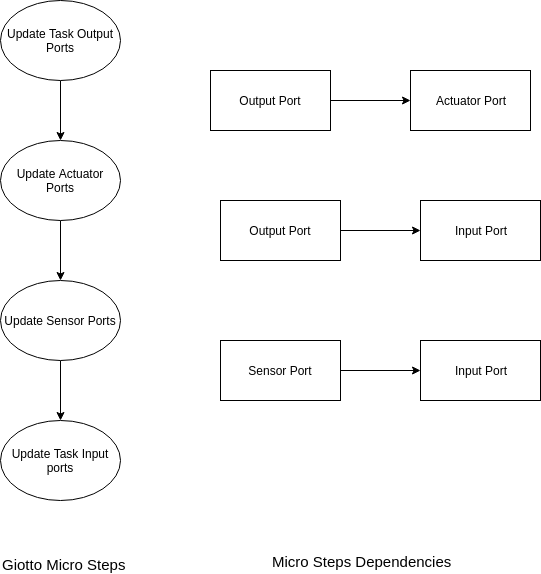
\includegraphics[width=\linewidth]{20MicroDepen.png}
\caption{Dependencies}
\end{figure}
There are only following data flow possible according to Giotto semantics:-
\begin{itemize}
    \item \textbf{Output Port to Actuator Port:-} Instance of task whose output port value is passed to some instance of actuator's port should be same as logical execution.
    \item \textbf{Output Port to Input Port:-} Instance of task whose output port value is passed to some instance of same or other task's input port should be same as logical execution.
    \item \textbf{Sensor Port to Input Port:-} Instance of senor's port whose value is passed to some instance of some task's input port should be same as logical execution.
\end{itemize}

\subsection{Explanation}
In actual execution all the data between the ports are flown only by means of driver. So we have to make sure the following :-
\begin{itemize}
    \item Instance of driver is associated with instance of task input port should be same as logical execution
    \item Instance of driver is associated with instance of task output port should be same as logical execution
    \item Instance of driver is associated with instance of sensor port should be same as logical execution
    \item Instance of driver is associated with instance of actuator port should be same as logical execution
\end{itemize}
\begin{figure}[H]
\centering
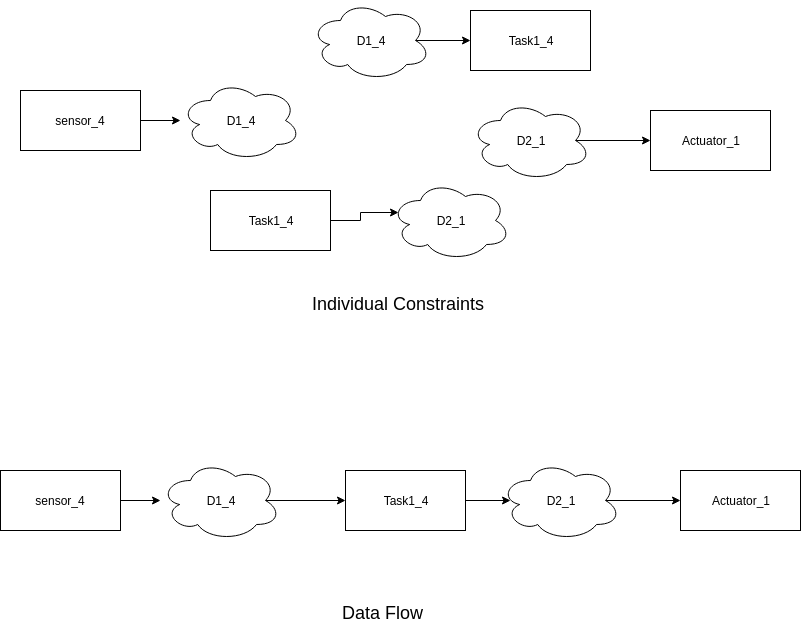
\includegraphics[width=\linewidth]{21DataFlow.png}
\caption{Data Flow}
\end{figure}
Data is passed inside and of task only by the means of its respective driver, so if we can add constraints to make sure that correct instance of driver pass value to correct instance of task and correct instance of driver receive value from correct instance of task we will get equivalent schedule. These constraints extraction are explained in more details in Chapter about Phase 2 Compiler.

\section{Reduction of TTProg Constraints to Z3 linear formulas}
Depending on the TTProg, large number of constraints can be generated which can be hard to solve. Z3 is a constraint solver which can solve a number of logical formulas. If the constraints are specifiable it will return \textbf{sat} and give the result for which it is being satisfied otherwise it will return \textbf{unsat}.\\
To be able to get a schedule if the result is sat we must be able to reduce all our constraints into linear Z3 formula. Reduction can be done as follows:-
\begin{itemize}
    \item All the instance of task and driver will become a constant of float time in Z3 and will represent the time at which that instance should start in a specifiable schedule. Example, t1\_0 = 3.4 means $0^{th}$ instance of task t1 should start at time 3.4 and should finish by its wcet
    \item All the instance of task and driver should be related to other instance of task or driver by means of their wcet and should be asserted to Z3 stack. Example $t1\_0 + wcet_{t1} <= d1_{2}$ , it means $0^{th}$ instance of task t1 should finish on or before the starting time of $2^{nd}$ instance of d1.
 \end{itemize}
For satisfiable schedule we will get start time of all the task and driver. Writing Z3 constraint are explained in more details in Chapter about Phase 2 Compiler.

\section{Timed Schedule to Timed Abstract Schedule}
For satisfiable schedule we will get a \textbf{timed schedule} similar to following example.
\begin{verbatim}
sat
[input_t2_2 = 8,
 input_t2_1 = 4,
 actuation_1 = 11,
 input_t2_0 = 1/2,
 t1_0 = 1/4,
 t2_0 = 1,
 actuation_0 = 5,
 t1_1 = 6,
 t2_1 = 25/4,
 input_t1_0 = 0,
 t2_2 = 17/2,
 input_t1_1 = 2]
\end{verbatim}

These timings are based on their wcet but these tasks and drivers execution will finish much before the wcet. So timing for all of the task and driver are not important. We will make a \textbf{Abstract Timed Schedule} which will be based on sorting all the task based start time. Abstract timed schedule still have to maintain the time for the following cases:-
\begin{itemize}
    \item Sensor read should occur at exact time range
    \item Actuator update should occur at exact time range
    \item Next mode cycle should start at exact time
\end{itemize}
Logically typical Abstract timed schedule will look like:-
\begin{verbatim}
    task1
    task2
    wait-till(5ms)
    sensor-read
    driver1
    task1
    wait-till(10ms)
    actuator-update
    task2
    wait-till(15ms)
\end{verbatim}
If the time period of mode is 15 it will repeat its execution after 15ms.

\section{Final Time Triggered Periodic Schedule}
In practice the logic for wait-till() is implemented by means of timer/counter interrupts. Clock ticks equivalent to the time is computed and timer/counter interrupt is set up.\\
Once a set of task and driver complete its execution it will go into busy wait until next interrupt is generated to schedule the sensor read or actuator update or new mode cycle along with next set of task.
It will do the following when interrupt is generated:-
\begin{itemize}
    \item Timer for next interrupt is
    \item A subset of Abstract timed schedule is deployed
\end{itemize}
It is explained in more detailed manned in Chapter about Phase 3 Compiler.


\chapter{Calculating the WCET}
WCET is the worst case execution time for each $Job \in \{Task, Driver\}$ that needs to be scheduled. WCET for each of task and drivers should be provided in the giotto.json program. The execution each Job may end before its WCET but in no case it should exceed the WCET time.\\
The WCET of a function can be computed by examining its machine code and knowing specification of time taken by the micro controller for each instruction. Due to complex control flow static analysis is used to come up with overestimation of WCET. The other technique is to experimentally measure WCET. This is used in our work.\\
To compute the WCET we need to take the difference of the end-timestamp and start-timestamp of the Job.

\begin{figure}[H]
\centering
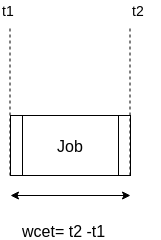
\includegraphics[width=0.3\linewidth]{17wcet.png}
\caption{Calculating WCET}
\end{figure}

To compute the WCET in Atmega 2560 we need to use timer/counters. We need to define an overflow interrupt to compute it. 

\section{Initializing Interrupts}
I have used timer 0 to calculate the WCET. Following is the initialization of timer 0 to compute the interrupts:-\\
\begin{verbatim}
    TCCR0A = 0;
    TCCR0B = (1 << CS00) | (1 << CS01) ;
    TIMSK0 = (1 << TOIE0);
\end{verbatim}

TCCR0A (Timer control register A) is set to 0, which sets WGM mode to Normal. In TCCR0B (Timer control register B) register CS00 and CS01 bits are set, which make the prescaler to 64. TIMSK0 (Timer Interrupt Mask register A) is set with TOIE0 which means the ISR will be called every time overflow occur in counter 0. Since timer 0 is a 8 bit counter overflow will occur after every 256 ticks.\\

\section{Using Prescaler 64}
Suppose $F\_CPU$ is the frequency of the CPU. And the prescaler value is $p$.
No of clock ticks per unit seconds will be:-
\begin{equation}
    \frac{F\_CPU}{p}
\end{equation}
Therefore, time for 1 tick will be :-
\begin{equation}
    \frac{p}{F\_CPU}
\end{equation}
In our case F\_CPU = 14745600 and p=64
\begin{equation}
    \frac{64}{14745600} = 4.34 \mu sec
\end{equation}
Since timer 0 is a 8 bit timer, the interrupt will occur after 256 ticks\\
\begin{equation}
    \frac{p}{F\_CPU}*Overflow\_ticks = 1.1111 ms
\end{equation}

\section{Defining the ISR}
The ISR function keeps track of the the number of number of overflows that are occuring in timer 0. The function will be as follows:-
\begin{verbatim}
volatile unsigned int timer0_overflow_count = 0; 
ISR(TIMER0_OVF_vect)
{
    timer0_overflow_count++;
}
\end{verbatim}

\section{micros() function}
micros() function will return the timestamp since the system is running in micro seconds. Difference between the two micros() function will determine the time elapsed between them. The function will be of the form:-
\begin{verbatim}
unsigned long micros()
{
    unsigned long m;
    unsigned char cnt;
    cli();
    cnt= TCNT0;
    m = (cnt + (timer0_overflow_count * 256))*4.34;
    sei();
    return m;
}
\end{verbatim}

Following formula is used to calculate the timestamp, total number of ticks are multiplied by time for each ticks:-
\begin{equation}
    timestamp = ( CounterValue + (NoOfOverflow * 256)) * EachTickTime
\end{equation}
Now execution time can be easily calculated as follows:-
\begin{verbatim}
t1=micros();
f1(1);
t2=micros();
time=(t2-t1);
\end{verbatim}
WCET value should be overestimate of this calculated time, say twice of this time.


\section{Limitations}
Following are the limitation of this approach:-
\begin{itemize}
    \item Since 1 tick time is $4.34 \mu sec$, the time computed will be a multiple of this time.
    \item ISR is called after every 1.11 ms on overflow, timer does not stop during serving of ISR. Therefor an error of 2\% is observed in the final computed value
    \item We cannot go for a lower prescaler value for better accuracy as it will increase the frquency of number of times ISR is called drastically, leading in large overhead
    \item By storing overhead count in a 16 bit integer we can computer the time upto 32 sec. By using 64 bit integer we can compute time in hours
\end{itemize}


\chapter{Phase 1 Compiler}
Phase 1 compiler is responsible for taking Firebird libraries, giotto\_input.h and giotto.josn as input and map these functions to the task and driver mentioned in giotto.json file. It will also auto generate all the port values as global variables and pass them as arguments to the Task and Drivers.

\begin{figure}[H]
\centering
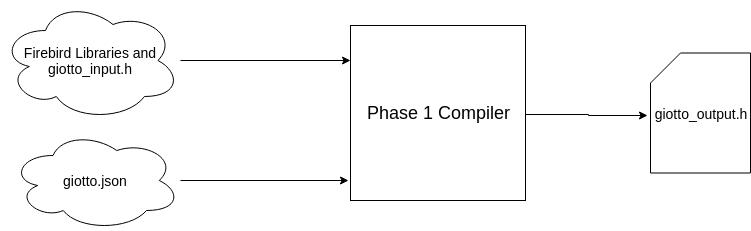
\includegraphics[width=\linewidth]{16phase1.png}
\caption{Phase 1 compiler}
\end{figure}

Any further stages to TTPorg program will only refer this giotto\_output.h file. Each function in this file will act as task and drivers.

\section{Algorithm}
\begin{itemize}
    \item It iterate through all the Input, Output, Actuator and sensor port and make global variable for them according to the type defined in the program
    \item It will then iterate through the all the task defined in the program:
    \begin{itemize}
        \item It will create a void function for all the task 
        \item It will create a mapping between the function name mentioned in the program and actual function definition by making the function call inside the task
        \item It will pass all the input port as the arguments and pass output ports as the pointer arguments so that a value can be returned
    \end{itemize}
    
    \item Similarly it will iterate through all the drivers defined in the program:
    \begin{itemize}
        \item It will create a void function for all the drivers 
        \item It will create a mapping between the function name mentioned in the program and actual function definition by making the function call inside the driver function
        \item It will pass all the input port as the arguments and pass output ports as the pointer arguments so that a value can be returned
    \end{itemize}
\end{itemize}

\section{Example}
Following is the sample giotto\_output.h:
\begin{verbatim}
#include "giotto_input.h"

//All ports as global variable

float s1;
float a=0;
float i1;
float i2;
float o1=0;
float o2=0;

//tasks as void functions
void t1(){
f1(i1,&o1);
}

void t2(){
f2(i2,&o2);
}


//drivers as void functions
void input_t1(){
h1(o2,&i1);
}

void input_t2(){
h2(&s1,&i2);
}

void actuation(){
h4(o1,&a);
}

\end{verbatim}


The TTProg program for the task t1 is as follows:-
\begin{verbatim}
    {"name" : "t1",
    "input" : ["i1"] , 
    "output": ["o1"], 
    "function":"f1", 
    "wcet":"0.25" }
\end{verbatim}
As we can is in above example the function f1 is called inside the task function t1. Its input port i1 is passed as an argument and its address of its output port o1 is passed.


\chapter{Phase 2 Compiler: TTProg Constraints}
\section{Functional Units of TTProg}
\begin{figure}[H]
\centering
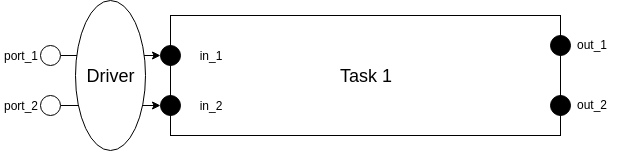
\includegraphics[width=0.9\linewidth]{1TaskSplit.png}
\caption{TTProg Task and Drivers}
\end{figure}

There are 2 functional Units in TTProg
\begin{itemize}
    \item Driver
    \item Task
\end{itemize}

\subsection{Driver}
There are 3 types of drivers in TTProg:
\begin{itemize}
    \item \textbf{Task Input} :- These divers provide value to task input port. Output to these diver are task output port. Input to these drivers may be constants, sensor value or output port value of some other task.
    \item \textbf{Actuator Update} :- These driver are responsible for actuation. Input to these drivers may be constants or output port value of some other task.
\end{itemize}

\subsection{Task}
Task reads value form input port associated with them. No two task can share input ports so input ports are unique to task. Task will to all the computation and will update its output port before finishing its execution.

% \section{Giotto Micro Steps}
% On working on single mode Giotto will have following 6 micro steps:-
% \begin{itemize}
%     \item \textbf{Update Task Ports :-} Output ports of previously completed task should be updated
%     \item \textbf{Update Actuator Ports :-} Once the task port is updated the dependent actuator are updated next
%     \item \textbf{Update Sensor Ports :-} Sensor read is performed and sensor port are updated next
%     \item \textbf{Update Task Input Ports :-} Input port of the task are then initialized by its drivers
%     \item \textbf{Update Active Task :-} No of task active are now updated
%     \item \textbf{Advance time :-} Time at which Giotto micro steps should execute next should be updated
% \end{itemize}

% \begin{figure}[H]
% \centering
% 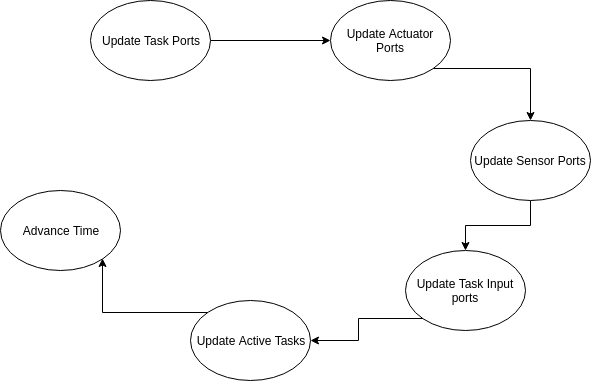
\includegraphics[width=\linewidth]{18microSteps.png}
% \caption{Giotto Micro Steps}
% \end{figure}

\section{Example of TTProg Execution}
\begin{figure}[H]
\centering
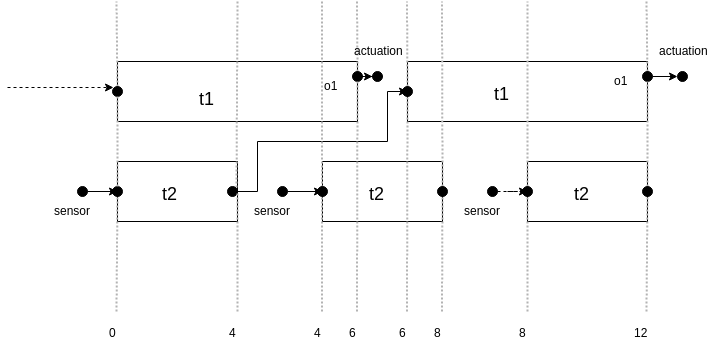
\includegraphics[width=0.9\linewidth]{2Example.png}
\caption{Sample Example}
\end{figure}


The above diagram is the logical execution of the TTProg program:-
\begin{verbatim}
    mode period 12
    task t1 driver input_t1 frequency 2
    task t2 driver input_t2 frequency 3
    actuator-driver act frequency 2
    jitter 1
\end{verbatim}

Input driver name for $t1$ is $input\_t1$ and input driver name for $t2$ is $input\_t2$. $act$ is the name of the actuator driver. Jitter tolerance is specified as 1 for sensor read and actuator update.

Let the program have following computed wcet(in ms): 
\begin{itemize}
    \item input\_t1 = 0.25
    \item t1 = 0.25
    \item input\_t2 = 0.5
    \item t2 = 1.0
    \item act = 1
\end{itemize}

\section{TTProg Constraints}
All the constraint are based on following assumptions. For $Job \in \{Driver,Task\}$:-
\begin{itemize}
    \item $job_{call}$ : The time at which the job should be called in final schedule is represented by name of the job and its instance as subscript. Example $t1_0$ will represent the time at which 0th instance of task t1 will start.
    \item $job_{return}$ : The time at which the job should finish its execution and return is assumed to occur before its wcet. Therefore, $t1_0$ should return before $t1_0 + wcet$  
\end{itemize}

Following will be the precedence and timing constraints according to Giotto semantics:- 
\subsection{Timing Constraints}
Giotto Semantics mandates actuator update and sensor read to occur at fixed time with some jitter tolerance.

\subsubsection{Actuator}

\begin{figure}[H]
\centering
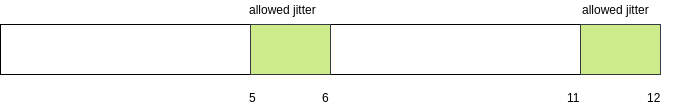
\includegraphics[width=0.9\linewidth]{3actJitter.png}
\caption{Actuator Jitter tolerance}
\end{figure}

In the above example actuator update must occur between the interval [6 - jitter  ,6] \& [12 - jitter , 12].\\
Let $i$ be the instance of the actuator task, formula for the constraints will be :
\textbf{Lower Bound:}
\begin{equation}
    actuation_i  >=  \frac{Mode Period}{Actuator Frequency}* i - jitter
\end{equation}
\textbf{Upper Bound:}
\begin{equation}
    actuation_i + wcet  <=  \frac{Mode Period}{Actuator Frequency}* i
\end{equation}

\noindent
\textbf{Example:}\\
    $actuation_0 >= 5$\\
    $actuation_0 + 1 <= 6$

\subsubsection{Sensors}
\begin{figure}[H]
\centering
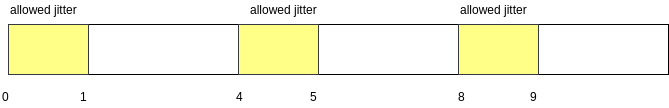
\includegraphics[width=0.9\linewidth]{4senJitter.png}
\caption{Sensor Jitter tolerance}
\end{figure}
Since input\_t2 is associated with a sensor read. Sensor read must occur between the interval [0 , 0 + jitter] , [4 , 4 + jitter] \& [8 , 8 + jitter]. \\
Let i be the instance of the task input which require sensor read, formula for constraints will be:\\
\textbf{Lower Bound:}
\begin{equation}
    input\_tn_{i}  >=  \frac{Mode Period}{TaskN Frequency}* i
\end{equation}
\textbf{Upper Bound:}
\begin{equation}
    input\_tn_{i} + wcet  <=  \frac{Mode Period}{TaskN Frequency}* i + jitter 
\end{equation}

\noindent
\textbf{Example:}\\
    $input\_t2_0 >= 0$\\
    $input\_t2_0 + 0.5 <= 1$

\subsubsection{Boundary Constraints}
These constraints make sure that all the task and drivers lies between the mode period.
For all, \\ $ Jobs \in \{ Task, Driver\} $ \\
$ Jobs >= 0$\\
$ Jobs <= ModePeriod $


\subsection{Precedence Constraints}
There are only 3 types of dependencies that we must maintain in order to keep values on the port consistent and get deterministic results:-
\begin{itemize}
    \item Task dependent on its input driver
    \item Actuator driver dependent on some task output
    \item Task input driver dependent on some other task output
\end{itemize}

\subsubsection{Precedence between Task and its Input Driver}
All the task its input driver for a task must occur before the task itself. Suppose task instance i is dependent on input driver instance i then any input driver instance i+1 should occur after task i.
It will be given to Z3 in the form \\
$input\_tn_i + wcet <= tn_i$ ,  where wcet is for the driver\\
$tn_i + wcet <= input\_tn_{i+1}$ , where wcet is for the task


\subsubsection{Actuator dependent on Task Output}
If input port of actuator driver is element of output port of some other task. We will first need to find the task on which it is dependent and then the instance $i$ of task on which it is dependent. Any instance $i+1$ on this task must occur after the actuation.

\begin{figure}[H]
\centering
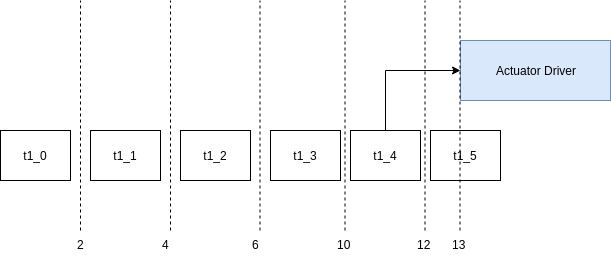
\includegraphics[width=0.9\linewidth]{6act.png}
\caption{Dependency according to logical execution}
\end{figure}

Above is the diagram show an example of logical execution of a Giotto program. To find out the task instance i on which Actuator Driver depend on according to logical execution we must divide the the time instance at which the Actuator is supposed to happen by the time period of task and take floor of it.
To add this as Z3 constraints we need to iterate through all the instance $actuation_i$ of the actuator driver. If task $t1_j$ is responsible for actuation \\
\begin{equation}
    j = \frac{Logical Start Time Of Actuation_i}{Logical Time Period Of t1}
\end{equation}
Constraints will be of form:\\
\textbf{Actuation i occur after task instance j}\\
$ t1_j + wcet_{task} <= actuation_i$\\
\textbf{Task instance j+1 should occur after the actuation}\\
$ actuation_i + wcet_{act} <= t1_{j+1}$\\

\noindent
If it is the last task execution the constraints will be only:\\
$ t1_j + wcet_{task} <= actuation_i$\\


\subsubsection{Task input driver dependent on some task output}
\begin{figure}[H]
\centering
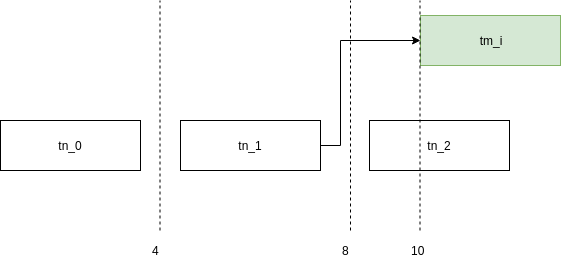
\includegraphics[width=0.9\linewidth]{7task.png}
\caption{Dependency according to logical execution}
\end{figure}

This case is also similar to actuator and task dependency. We first need to find if for some task t1 \& t2  , if t2 output port is used by input driver of t1. We will find the instance $j$ of t2 which should occur before input driver of instance $i$ of t1, using the formula:
\begin{equation}
    j = \frac{Logical Start Time Of t1_i}{Logical Time Period Of t2}
\end{equation}
\noindent
Constraints will be of form:\\
\textbf{To make sure first call of t1 take value from last mode call}\\
$ input\_t1_0 + wcet_{t1}  <= t2_0$\\
\textbf{Instance i of t1 should occur after instance j of t2}\\
$t2_j + wcet_{t2} <= input\_t1_i$\\
\textbf{To make sure other instance of t2 run after input driver of $t1_i$}\\
$input\_t1_i + wcet_{input\_t1} <= t2_{j+1}$

\subsubsection{Ordering of instances of Task}
For all task tn and its instances $tn_i$ \& $tn_{i+1}$.\\
$tn_i + wcet <= tn_{i+1}$

\subsection{Some extra Constraints for Z3}
\subsubsection{Serialization Constraints}
There might still be many task and drivers between which there are no dependencies. These constraints ensures that at most one job executes at a time i.e.  new job is scheduled only after completion of previous job's wcet. This confirms to uni-processor architecture. Each job runs automatically without any preemtion.
For all possible\\
$job_1 , job_2 \in \{Drivers, Task\}$\\
$job_1 != job_2$\\
Constraints will be of form:\\
$ job_1 + wcet_1 <= job_2 || job_2 + wcet_2 <= job_1$\\\\
It will make sure that either $job_1$  occur before $job_2$ or after it and does not overlap.

\section{Result}
Once all the constraints generated it is stored in a file. Python API of Z3 is used to add all assertions with the help of another script.
On successful execution z3 gives the result as follows:
\begin{figure}[H]
\centering
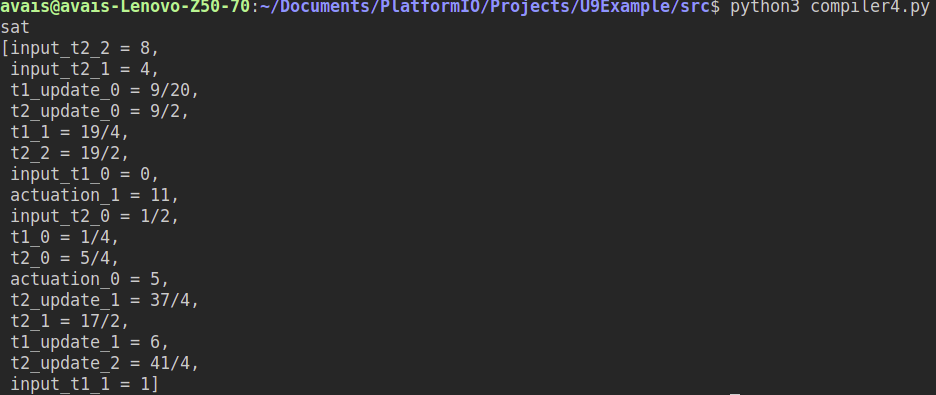
\includegraphics[width=1\linewidth]{8ss.png}
\caption{Result}
\end{figure}
Above schedule is a valid Giotto execution. This timed schedule is again stored in a file for code generation.
Note that this is only one of the possible schedules meeting the constraints.

\chapter{Phase 3 Compiler: Generating the C-code using the schedule}
After the previous phase compilation Z3 will give us the time which contains the name of instances of task and driver and the time at which it shout start its execution.

\begin{figure}[H]
\centering
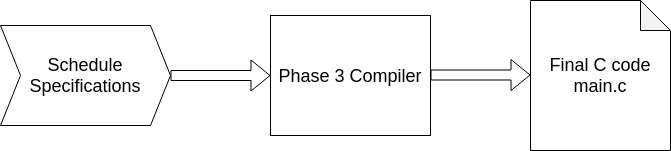
\includegraphics[width=1\linewidth]{11phase3.png}
\caption{Phase 3 Compiler}
\end{figure}

A sample of the schedule specification obtained from example shown in Fig.7.2 is :-
\begin{verbatim}
sat
[input_t2_2 = 8,
 input_t2_1 = 4,
 actuation_1 = 11,
 input_t2_0 = 3/10,
 t1_0 = 1/4,
 t2_0 = 4/5,
 actuation_0 = 5,
 t1_1 = 6,
 t2_1 = 9/2,
 input_t1_0 = 0,
 t2_2 = 17/2,
 input_t1_1 = 9/5]
\end{verbatim}
Z3 first specify weather it is sat or unsat. If it is sat it will provide start time for each $Job\_instance$ where $Job \in \{Task, Driver\}$.\\
This phase of compilation will take this schedule specification as input and will generate a C-code which is equivalent to this schedule.

\section{Idea}
The main.c generated will implement the idea of Cooperative multitasking. It is a non-preemptive that will update the schedule based in timer interrupts. I have reserved Timer/Counter 4 of Atmega 2560 for this operation.\\
The main.c generated will be of form:-
\begin{verbatim}
int main(int argc, char *argv[])
{
    //initializing the counter interrupt 4
    schedule = 1;
    isr_schedule = 1;
    while (1)
    {
        switch (schedule)
        {
        case 0:
            schedule = 0;
            break;
        case 1:
            task1();
            task2();
            driver1();
            .
            .
            schedule = 0;
            break;
        case 2:
            driver1();
            task1();
            task2();
            .
            .
            schedule = 0;
            break;
        case 3:
            driver1();
            driver2();
            .
            .
            schedule = 0;
            break;
        case 4:
            actuation();
            task1()
            .
            .
            schedule = 0;
            break;
        .
        .
        .
        }
    }
    return 0;
}

// Interrupt Servive routine to schedule the task
ISR(TIMER4_COMPA_vect)
{
    switch (isr_schedule)
    {
    case 1:
        OCR4A = 1021;
        schedule = 2;
        isr_schedule = 2;
        break;
    case 2:
        OCR4A = 1252;
        schedule = 3;
        isr_schedule =3;
        break;
    .
    .
    .
    .
    case 6:
        OCR4A = 169;
        schedule = 1;
        isr_schedule =1;
        TCNT4 = 100;
        break;
    }
}
\end{verbatim}

\subsubsection{Schedule Case}
According to TTProg Semantics the sensor read and actuator update are meant to happen on specific time within the Jitter Tolerance. To achieve this the final schedule is dividend into many smaller schedule cases based on start time of sensor read and actuator update.

\begin{figure}[H]
\centering
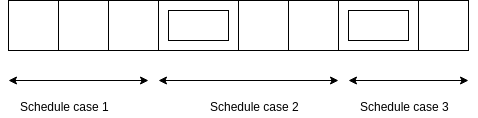
\includegraphics[width=1\linewidth]{13SchDivision.png}
\caption{Schedule case Division}
\end{figure}

In the above diagram double box represents sensor read or actuator update which are meant to happen at specific time. New smaller schedule case starts from such sensor or actuator jobs until next actuator or sensor job.\\
Each of these smaller schedule case can be referred using switch case in the in the main function.\\
Task and drivers are scheduled by means of direct function call. The functions are called in the order in which they are supposed to be scheduled inside switch case. By the end of each schedule case the program goes back to busy waiting until an interrupt is generated to schedule the next schedule case.

\begin{figure}[H]
\centering
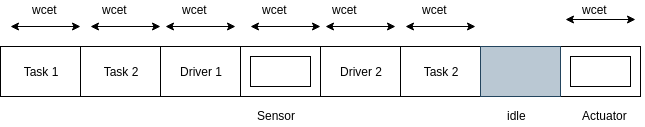
\includegraphics[width=1\linewidth]{12scheduling.png}
\caption{Schedule Example}
\end{figure}

The Jobs are assumed to run no longer than time specified by wcet. Jobs can finish much sooner than wcet. In that case the CPU will go to busy wait at the end of each schedule case until the interrupt to deploy next schedule case is generated. It will cause no effect on schedule logically and the result will be equivalent.

\begin{figure}[H]
\centering
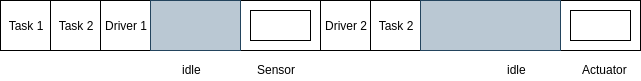
\includegraphics[width=1\linewidth]{12scheduling2.png}
\caption{Equivalent Schedule}
\end{figure}

Case 0 of the switch is used to perform the busy waiting. Once any schedule case have completed its execution it will go back to case 0 for busy waiting.\\
The final schedule will be series if schedule case which are followed busy waiting until an interrupt is generated to deploy next schedule case. The overall schedule will keep repeating itself over the time defined by mode period. 

\begin{figure}[H]
\centering
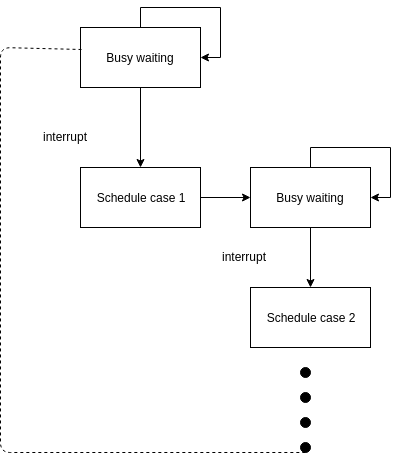
\includegraphics[width=0.7\linewidth]{14execution.png}
\caption{Schedule Execution}
\end{figure}

\subsubsection{Interrupts}
The ISR plays an important role in this scheduling to make sure that sensor read and actuator update run at specific time. We are Timer 4 of Atmega 2560 for scheduling. The global variable $isr_schedule$  keep track about which schedule case is currently in execution. Following will happen whenever an interrupt happens:-
\begin{itemize}
    \item It will first check which is the current schedule case
    \item It will update the time at which next timer interrupt should occur
    \item It will update the value of $schedule$ variable such that next schedule case can be deployed
    
\end{itemize}

\section{Algorithm and Technicalities}
\begin{figure}[H]
\centering
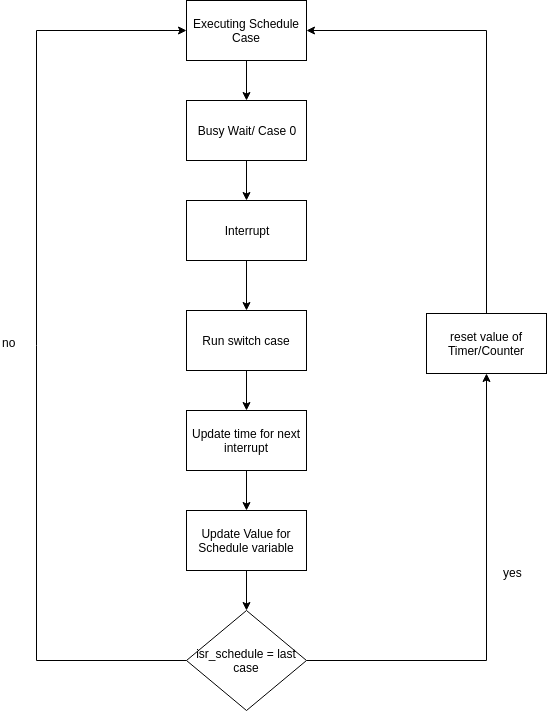
\includegraphics[width=\linewidth]{15flowChart.png}
\caption{Flow}
\end{figure}
To sum up the overall flow will be as follows:-
\begin{itemize}
    \item The main program will start with first schedule case as being currently scheduled. The time for the first interrupt will also be initialized.
    \item It will complete execution of all the jobs and will to busy wait on schedule 0
    \item Once the first interrupt occur, it will go to the code block inside switch case according to the currently running switch case
    \item This ISR's code block will first update time for next interrupt
    \item It will update value for $schedule$ variable so that next schedule case can be deployed
    \item It will check if it is the last case of the mode, if it the last case it will reset the value for Timer/Counter 4, so that the cycle can repeat itself
    \item A new schedule case will be deployed
\end{itemize}

\subsection{Timer/Counter 4}
Firebird V contains a Atmega 2560 master processor and a Atmega 8 slave processor. We will be using Timer/Counter 4 of Atmega 2560 to synchronize the scheduling.
Timer/Counter 4 is a 16 bit counter i.e. it overflows after 65536 ticks.\\
\textbf{Timer/Counter 1 Control Register A (TCCR4A)} is set with WGM4x bits are set to 0 for normal operation.\\
\textbf{Timer/Counter 1 Control Register B (TCCR4B)} is set with CS00 and CS01 bits to set prescaler value to 64. The prescaler value will divide the clock by a given factor, now for ever 64 ticks the counter value will increase by 1 tick. By changing the prescaler value we can increase/decrease the total time after which counter overflows.\\
\textbf{Timer/Counter 4 Interrupt Mask Register(TIMSK4)} is set with OCIE4A bit, which will trigger the interrupt when the counter value matches with OCR4A register value.
Following code will initialize the Timer 4 as required by the scheduler:-

\begin{verbatim}

    //Waveform Generation Mode is normal
    TCCR4A = 0;
    
    //setting prescaler to 64
    TCCR4B = (1 << CS00) | (1 << CS01); 
    
    //Setting timer mask register to 
    //Output Compare A Match Interrupt Enable mode
    TIMSK4 = (1 << OCIE4A);
    
    //Initial value for compare register
    OCR4A = 169;
\end{verbatim}

\subsubsection{Computing time based on clocks}
Time for each interrupt is used in main code in the form of counter value which is based on $clk/prescaler$ value.
Atmega 2560 used in firebird run at the frequency of 14745600 Hz. The formula for converting the actual time in ms obtained from Z3 to clock tick time is :-
\begin{equation}
    ticks = \frac{F\_CPU}{Prescaler} * Time
\end{equation}

In our case $F\_CPU$ is 14745600 Hz. $Prescaler$ is 64 and $Time$ is given by Z3 in milli seconds.

\subsubsection{Limitations}
This approach of scheduling have following limitation:-
\begin{itemize}
    \item It reserves a Timer and is cannot be used in other operations
    \item The mode period cannot exceed the overflow value of the timer. In our case it is predefined to 284ms based on the prescaler 64 value.
    \item The scheduler may lose the precision if we further increase the prescaler value
\end{itemize}

\subsection{Compiler Algorithm}
The compiler works based on following algorithm:-
\begin{itemize}
    \item It parse the schedule generated by Z3.
    \item It then sort all the task instance according to time at which its execution is supposed to start
    \item The compiler will read the giotto.json file to find which of the driver are responsible for the sensor read or actuator update
    \item It will then prepare a dictionary with the name of driver associated with sensor read and actuator update and its clock time. This is the time at which all the interrupt should occur
    \item The compiler will make the function call for all the task and driver in the main function
    \item The compiler will make separate switch case whenever a driver needs to be scheduled which is responsible for interrupt.
    \item Similar approach is used to make the ISR function. The interrupt dictionary is used to set the value at which next interrupt needs to occur
\end{itemize}

\section{Example}
For the example shown in Fig.7.2 the final C-code will be:-

\begin{verbatim}
#include "giotto_output2.h"
volatile unsigned int schedule = 0;
volatile unsigned int isr_schedule = 0;
int main(int argc, char *argv[])
{
    init_devices();
    TCCR4A = (1 << WGM42);
    TCCR4B = (1 << CS00) | (1 << CS01);
    TIMSK4 = (1 << OCIE4A);
    OCR4A = 169;
    schedule = 1;
    isr_schedule = 1;
    while (1)
    {
        switch (schedule)
        {
        case 0:
            break;
        case 1:
            input_t1();
            t1();
            schedule = 0;
            break;
        case 2:
            input_t2();
            t2();
            input_t1();
            schedule = 0;
            break;
        case 3:
            input_t2();
            t2();
            schedule = 0;
            break;
        case 4:
            actuation();
            t1();
            schedule = 0;
            break;
        case 5:
            input_t2();
            t2();
            schedule = 0;
            break;
        case 6:
            actuation();
            schedule = 0;
            break;
        }
    }
    return 0;
}
ISR(TIMER4_COMPA_vect)
{
    switch (isr_schedule)
    {
    case 1:
        OCR4A = 1021;
        schedule = 2;
        isr_schedule = 2;
        break;
    case 2:
        OCR4A = 1252;
        schedule = 3;
        isr_schedule = 3;
        break;
    case 3:
        OCR4A = 1943;
        schedule = 4;
        isr_schedule = 4;
        break;
    case 4:
        OCR4A = 2634;
        schedule = 5;
        isr_schedule = 5;
        break;
    case 5:
        OCR4A = 2864;
        schedule = 6;
        isr_schedule = 6;
        break;
    case 6:
        OCR4A = 169;
        schedule = 1;
        isr_schedule = 1;
        TCNT4 = 100;
        break;
    }
}

\end{verbatim}


\chapter{Case Study}

\section{Introduction}
We will use a simple example to demonstrate working of TTProg[Heptagon]. We will build Adaptive Cruise control along with Parking Detect. The following two Heptagon components will be combined using TTProg:-
\begin{itemize}
    \item \textbf{Adaptive Cruise control} :- It will follow the white line and if an obstacle is detected it will first reduce the speed and then stop.
    \item \textbf{Parking Detect} :- It will keep checking for free space on the right, if a space around 5 cm is detected the robot will slow down and sound the buzzer.
\end{itemize}

\section{Heptagon Node}
We will use two Heptagon nodes and generate its C-code with the heptagon compiler to provide input to TTProg. 
Heptagon Node for Adaptive Cruise control will be as follows:-
\begin{verbatim}
    node acc(blocked,leftOut,rightOut,centreOut : bool; rightBlock : int) 
    returns (wheelLeft,wheelRight : int);
let
      wheelLeft= if blocked=true or rightBlock=0 then 0
                else if(centreOut = false) then 3
                else if(centreOut = true and leftOut =true 
                        and rightOut=true) then 0
                else if rightOut=true then 1
                else if leftOut=true then 2 else 0;

      wheelRight= if blocked=true or rightBlock=0 then 0
                else if(centreOut = false) then 3
                else if(centreOut = true and leftOut =true 
                        and rightOut=true) then 0
                else if rightOut=true then 2
                else if leftOut=true then 1 else 0;

tel
\end{verbatim}
This implementation set the speed of left wheel and right wheel in the scale of 0,1,2 and 3. The input parameter are provided by the input driver as follows:-
\begin{itemize}
    \item \textbf{blocked} = Will be true if front is blocked
    \item \textbf{leftOut} = Will be true when left white line sensor is not on white line
    \item \textbf{rightOut} = Will be true when right white line sensor is not on white line
    \item \textbf{centerOut} = Will be true when center white line sensor is not on white line
    \item \textbf{rightBlock} = Will be 0 if space for parking is detected
\end{itemize}


\vspace{5mm}
\noindent
Heptagon Node for Parking Detect will be as follows:-
\begin{verbatim}
node park(rf,rb : int) returns (rightBlocked : int);
let

      rightBlocked = if (rf > 150 and rb > 100) then 0 
                    else 1;
tel
\end{verbatim}

The input parameter are provided by the input driver as follows:-
\begin{itemize}
    \item \textbf{rf} = It is the sensor value of the front sensor on the right side of firebird robot
    \item \textbf{rb} = It is the sensor value of the back sensor on the right side of firebird robot
\end{itemize}
If the values satisfies $rf > 150$ \& $rb > 100$ then we can conclude that there is free space on the right side for parking otherwise blocked.

\section{TTProg Logical Execution}
We need to specify wcet for each of our task and driver in our TTProg specification. All the wcet are overestimated in this example. Time period of the mode is 16 ms.

\begin{figure}[H]
\centering
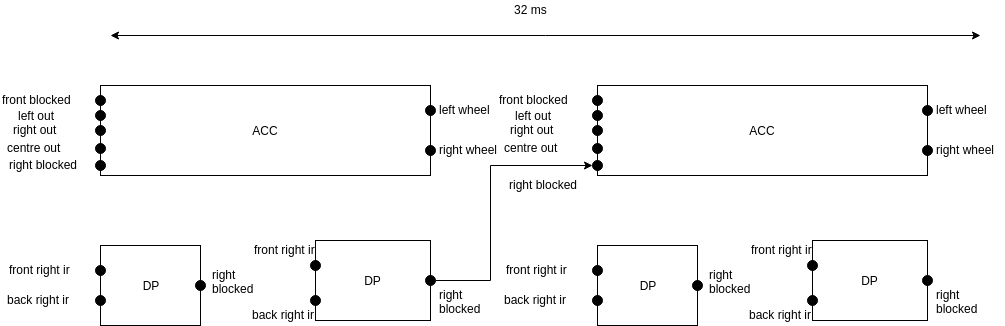
\includegraphics[width=\linewidth , height= 6cm]{22ttprogExp.png}
\caption{TTProg Execution}
\end{figure}

Task DP is Detect Parking and Task ACC is Adaptive Cruise Control.
All the input port value is provided by means of sensor read except input port $right-blocked$ of ACC which is provided by task DP.
Task ACC is responsible for controlling the left wheel and right wheel as actuator update , on other hand task DP control buzzer as actuator update.\\
giotto.json file will look as follows:-
\begin{verbatim}
    {
    "sensor" : [
        {"name" : "FrontBlocked" , "type" : "float"},
        {"name" : "leftOut" , "type" : "float"},
        {"name" : "rightOut" , "type" : "float"},
        {"name" : "centreOut" , "type" : "float"},
        {"name" : "frontRightIR" , "type" : "float"},
        {"name" : "backRightIR" , "type" : "float"}
    ],

    "actuator" : [
        {"name" : "wheel" , "type" : "float" , "init" : "0"},
        {"name" : "buzzer" , "type" : "float" , "init" : "0"}
    ],
    
    "input" : [
            {"name" : "FrontBlockedi" , "type" : "float"},
            {"name" : "leftOuti" , "type" : "float"},
            {"name" : "rightOuti" , "type" : "float"},
            {"name" : "centreOuti" , "type" : "float"},
            {"name" : "frontRightIRi" , "type" : "float"},
            {"name" : "backRightIRi" , "type" : "float"},
            {"name" : "rightBlockedi" , "type" : "float"}
    ],

    "output" : [
        {"name" : "leftWheel", "type" : "float" , "init": "0"},
        {"name" : "rightWheel", "type" : "float" , "init": "0"},
        {"name" : "rightBlocked", "type" : "float" , "init": "0"}
    ],

    "private" : [
    ],

    "task" : [
        {"name" : "t1", 
        "input" : ["FrontBlockedi","leftOuti","rightOuti",
                    "centreOuti","rightBlockedi"] ,
        "output": ["leftWheel","rightWheel"], 
        "function":"Cor__acc_step", "wcet":"2" },
        {"name" : "t2", "input" : ["frontRightIRi","backRightIRi"] , 
        "output": ["rightBlocked"], "function":"RightO__rightO_step", 
        "wcet":"1" }
    ],

    "driver" : [
        {"name" : "input_t1", 
        "input" : ["FrontBlocked","leftOut","rightOut",
                "centreOut","rightBlocked"] , 
        "output": ["FrontBlockedi","leftOuti","rightOuti",
                "centreOuti","rightBlockedi"], 
        "function":"inputDriver",  "wcet":"1" },
        {"name" : "input_t2", "input" : ["frontRightIR","backRightIR"] ,
        "output": ["frontRightIRi","backRightIRi"], 
        "function":"inputDriver2", "wcet":"0.5" },
        {"name" : "actuation", "input" : ["leftWheel","rightWheel"] ,
        "output": ["wheel"], "function":"actDriver" , "wcet":"1" },
        {"name" : "actuation2", "input" : ["rightBlocked"] , 
        "output": ["buzzer"], "function":"actDriver2", "wcet":"0.5" }

    ],

    "mode" : [
        {"name" : "m1", "period" : "16" ,  "definition":[
            {"type": "sensor", "frequency": "1", "task": "t1", 
            "driver": "input_t1"},
            {"type": "actuator", "frequency": "1", "driver": "actuation"},
            {"type": "sensor", "frequency": "2", "task": "t2", 
            "driver": "input_t2"},
            {"type": "actuator", "frequency": "2", "driver": "actuation2"}
        ]}
        ],
    "jitter" : "2"
}
\end{verbatim}


\section{Physical Schedule}

Final Execution will have schedule of the form:-
\begin{figure}[H]
\centering
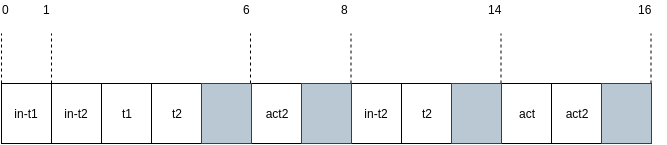
\includegraphics[width=\linewidth ]{23scheduleEx.png}
\caption{TTProg Execution}
\end{figure}
Grey boxes will indicate busy wait and interrupt will be generated at the time signified by the dotted line.\\


Its C-code will be as follows:-

\begin{verbatim}
#include "giotto_output2.h"
volatile unsigned int schedule = 0;
volatile unsigned int isr_schedule = 0;
int main(int argc, char *argv[])
{
    init_devices();
    \\init for timer
    TCCR4A = 0;
    TCCR4B = (1 << CS00) | (1 << CS01);
    TIMSK4 = (1 << OCIE4A);
    OCR4A = 330;
    
    schedule = 1;
    isr_schedule = 1;
    while (1)
    {
        switch (schedule)
        {
        case 0:
            break;
        case 1:
            input_t1();
            schedule = 0;
            break;
        case 2:
            input_t2();
            t1();
            t2();
            schedule = 0;
            break;
        case 3:
            actuation2();
            schedule = 0;
            break;
        case 4:
            input_t2();
            t2();
            schedule = 0;
            break;
        case 5:
            actuation();
            schedule = 0;
            break;
        case 6:
            actuation2();
            schedule = 0;
            break;
        }
    }
    return 0;
}
ISR(TIMER4_COMPA_vect)
{
    switch (isr_schedule)
    {
    case 1:
        OCR4A = 1482;
        schedule = 2;
        isr_schedule = 2;
        break;
    case 2:
        OCR4A = 1943;
        schedule = 3;
        isr_schedule = 3;
        break;
    case 3:
        OCR4A = 3325;
        schedule = 4;
        isr_schedule = 4;
        break;
    case 4:
        OCR4A = 3556;
        schedule = 5;
        isr_schedule = 5;
        break;
    case 5:
        OCR4A = 3786;
        schedule = 6;
        isr_schedule = 6;
        break;
    case 6:
        OCR4A = 330;
        schedule = 1;
        isr_schedule = 1;
        TCNT4 = 100;
        break;
    }
}

\end{verbatim}

\section{Results}
The above C-code was able to successfully compile and build for FireBird V. A .hex file is generated on build which is then loaded to the Robot. It was observed that the robot was successfully able to perform desired functionality. Thus, we have demonstrated the applicability of our TTProg[Heptagon] High Level Programming technique to robotics.



\chapter{Conclusion}
% The abstraction provided by programming languages like Giotto and Heptagon made it much simpler to use. The component based design make it possible to reuse a certain functionality with ease. The Giotto[Heptagon] model which is based on GALS provide a high level language for the coordination of embedded systems like Fire Bird V robot.
Our time triggered program framework facilitates us to easily schedule complex task structure. It eliminated the limitations of powerful synchronous languages like Heptagon by allowing time intensive task. \\
The user don't need to worry about scheduling the task, he only need to provide the functions as input and specify the logical execution. It is architecture and processor independent. The automated compiler automatically checks if it is feasible to schedule and generate a C-code for the schedule.\\
Its Disadvantage is that WCET of each task has to be measured and provided. Long tasks have to be manually broken into sequence of small tasks which can be statically scheduled automatically.\\ This allow us to eliminate need for context switching or memory allocation. Hence very efficiently executable code is obtained. 
\section{Future Work}
Following are the future work that can be done:-
\begin{itemize}
    \item Handling multiple mode and mode switch of Giotto semantics
    \item Giving an option to user to choose various Timer and prescaler value for scheduler according to his need
    \item Error handling to done in compiler
    \item Method can be extended to using multi-processor systems
    
    \newpage
    
    \item Automatic technique for decomposing long functions into a chain of small atomic task need to be developed
    \item Method needs to be applied to complex robot programming e.g. control of humanoid robots
\end{itemize}


\bibliographystyle{plain}
\renewcommand{\bibname}{References}
\bibliography{lab}
\begin{thebibliography}{9}
\bibitem{giotto} 
Thomas A. Henzinger, Benjamin Horowitz and Christoph M. Kirsch,
"Giotto: A Time-triggered Language for Embedded Programming", in Proceedings of the IEEE, vol. 91. IEEE, 2003

 
\bibitem{chart} 
David Harel, ”Statecharts: A visual formalism for complex systems”, in Science of Programming, vol. 8. Elsevier, 1987.


\bibitem{linda} 
George Wells, "Coordination Languages: Back to the Future with Linda" in Proceedings of WCAT’05. 2005


\bibitem{lustre}
Pascal Raymond and Nicolas Halbwachs, "The Lustre Language". URL: http://www-verimag.imag.fr/~raymond/edu/eng/lustre-a.pdf

\bibitem{heptagon} 
Heptagon/BZR manual. 2017. URL : \url{http://heptagon.gforge.inria.fr/pub/heptagon-manual.pdf}

\bibitem{fb} 
Fire Bird V Software and Hardware manual. URL : \url{http://elsi.e-yantra.org/resources}

\bibitem{z} 
Z3 - Guide by Microsoft. URL : \url{https://rise4fun.com/z3/tutorial}

\bibitem{atmega} 
ATmega-2560 Datasheet. URL:\url{https://ww1.microchip.com/downloads/en/devicedoc/atmel-2549-8-bit-avr-microcontroller-atmega640-1280-1281-2560-2561\_datasheet.pdf}

\bibitem{yakindu}
Yakindu Statechart Tool. URL: \url{https://www.itemis.com/en/yakindu/state-machine/}


\end{thebibliography}

\end{document}

